\section{Introduction to GPU computing (2)}

\begin{figure}[htbp]
    \begin{minipage}[c]{0.55\textwidth}
        Now that we know what a GPU is, let's introduce some more accurate terminology. First of all, the GPU will be connected to your computer through the so called \textbf{Bus PCI Express} on your mother board. We are going to call \textbf{host} the computer to which the GPU is connected and \textbf{device} the GPU itself. The host contains the CPU and the RAM: the serial part of our programs is going to run on that. The part of our code that runs on the GPU is called the \textbf{kernel} and its execution consists in 3 main steps:
        \begin{enumerate}
            \item copy the data from the host (hard disk or RAM) to the device;
            \item copy the kernel and execute;
            \item copy back results.
        \end{enumerate}
        With that said, what is \textbf{CUDA}?  It is a set of C/C++ extensions to enable GPU computing on NVIDIA GPUs. In other words, it is a framework that enables you to go through all those 3 phases of execution. Dedicated APIs allow to control almost all the functions of the graphics processor.
    \end{minipage}\hfill 
    \begin{minipage}[c]{0.42\textwidth}
        \centering
        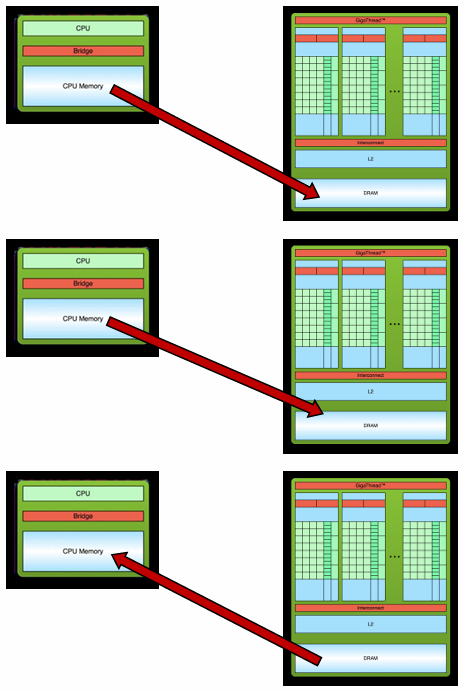
\includegraphics[width=\textwidth]{figuresP/lesson_parallel_4_pag_3.png}
    \end{minipage}
\end{figure}

\subsection{Blocks $\rightarrow$ multiprocessors , threads $\rightarrow$ cores}
Take a look at the schematic representation of a GPU below.

\begin{center}
    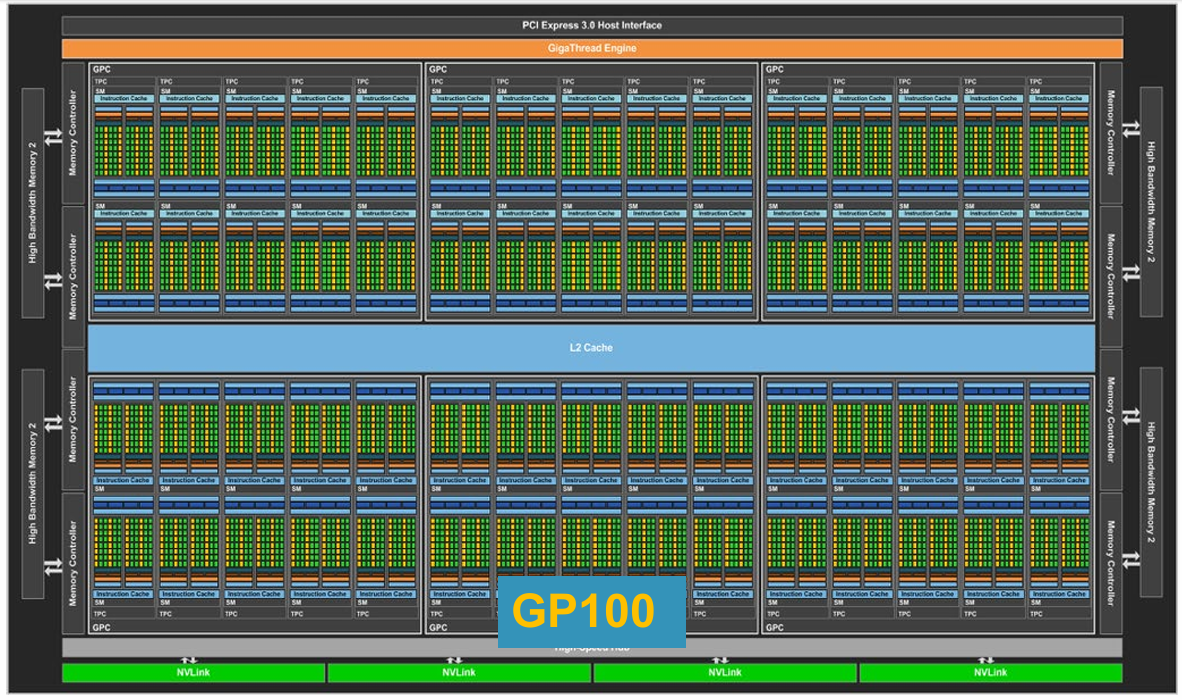
\includegraphics[width=\textwidth]{figuresP/lesson_parallel_4_pag_5.png}
\end{center}

As said before, a GPU is composed of simpler structures called \textbf{multiprocessors} that contain a grid of cores. Each multiprocessor has a SIMD architecture, so each core must execute the same instruction, but different multiprocessors can execute different parts of the program (SIMT). Take a look at the physical structure of a multiprocessor in the figure below.

\begin{center}
    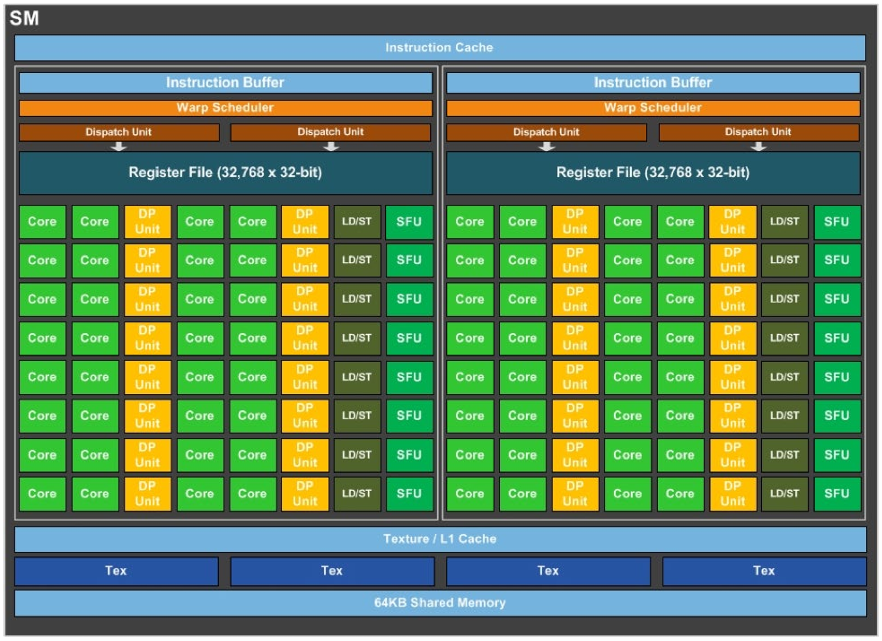
\includegraphics[width=0.8\textwidth]{figuresP/lesson_parallel_4_pag_6.png}
\end{center}

There is an important analogy between how a GPU is physically built and how a program that is supposed to run on it can be organized. A group of threads that can communicate and synchronize (i.e. execute the same instruction at the same time) is called a \textbf{block} (and a group of block is called a \textit{grid}). Threads in different blocks do not interact. 

To understand this concept let's imagine a simple situation. Let's say that we have a GPU with 1000 cores grouped in 10 multiprocessors. Intuitively, one could say that on this GPU you can run 10 blocks with 100 threads each, but that would be wrong. \\ Inside each multiprocessor there is a component called \textbf{instruction buffer} or "\textbf{small scheduler}". If each block contains 300 threads, the scheduler will send the first 100 threads to the cores to be executed and then the remaining 200 to the cores that concluded their execution. \\ Similarly, a GPU must have a "\textbf{big scheduler}" that distributes blocks to the multiprocessors in the same way. The terms "small" and "big" come from the fact that the GPU scheduler can manage thousands of billions of blocks, while the multiprocessor one is usually limited to 2048 threads at a time. \\ That means that the analogy "threads $\rightarrow$ cores" and "blocks $\rightarrow$ multiprocessors" is of course not perfect, since a GPU can manage a much larger number of blocks than the number of multiprocessors it has.  

\subsection{Memory hierarchy}

As we can observe from the architectural schematics above, understanding the memory hierarchy is fundamental in GPU programming. Unlike modern CPUs, where caching is mostly transparent, on a GPU a significant portion of memory management and data locality optimization is explicitly left to the programmer. Memory is structured into a hierarchy based on physical location, speed, and scope:

\begin{itemize}
    \item \textbf{Global Memory}: This is the main memory of the GPU (labeled as \textit{High Bandwidth Memory} on in the GPU figure above). It is located "off-chip" on the GPU board, meaning it has the highest latency and is relatively slow. However, it is vast, lasts for the entire lifetime of the application, and is universally accessible: both the host and all threads across all grids on the device can read and write to it. As seen in the first figure, accesses to global memory are typically buffered through a large, shared \textbf{L2 Cache} located in the centre of the GPU.
    
    \item \textbf{Shared Memory}: Looking at the multiprocessor diagram, you can clearly spot a dedicated block labeled \textit{64KB Shared Memory} at the bottom. Because it resides directly "on-chip" within the multiprocessor, it is extremely fast. This memory is allocated \textit{per-block}: it is readable and writable by all threads within the same block, allowing them to synchronize and share data efficiently. Its lifetime is tied strictly to the execution of that specific block.
    
    \item \textbf{Registers (Private Memory)}: The same figure also prominently features massive \textit{Register Files} (e.g., $32,768 \times 32$-bit) sitting right above the processing cores. Registers represent the fastest type of memory available. They are allocated on a \textit{per-thread} basis. The data stored here is strictly private, meaning it is only readable and writable by the individual thread that owns it, and its scope lasts only for the lifetime of that single thread.
\end{itemize}

The problem is that memory transfer is comparably slow. The solution is to do something else in the meantime, like some more computation. You can overlap tasks by having copy and compute engines run separately (\textit{asynchronicity}). The CPU can do other work while the GPU computes, handling synchronization when needed. This will work only on modern GPUs and we will not dive deeper into this method. 

\begin{center}
    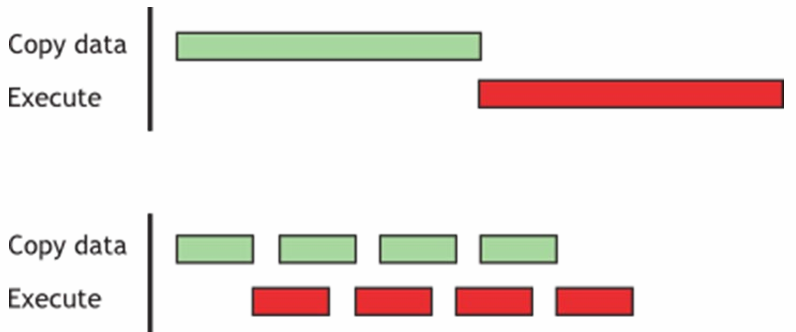
\includegraphics[width=0.4\textwidth]{figuresP/lesson_parallel_4_pag_8.png}
\end{center}

\subsection{How to program a GPU?}

There are entire courses and books dedicated to GPU programming. Here you are going to get the general idea and learn the basics that are imperative if you want to delve deeper into the topic in the future.

CUDA is the "best" way to program NVIDIA GPUs at a low level. If your code is almost all CPU (as in many applications to data analysis in physics) or if you need to accelerate dedicated functions, you could consider using \textit{directives} (OpenMP, OpenACC) or \textit{libraries} (Thrust, ArrayFire, cuBLAS, cuFFT, etc.). These tools lets you use the GPUs at a high level, sometimes without even knowing it. OpenCL is a framework equivalent to CUDA used to program multiplatforms (GPU, CPU, DSP, FPGA). C/C++ and Fortran are the "official" languages for CUDA, while Python and other languages are supported through wrapping and libraries (like Numba, PyCUDA, Theano).

Take a rapid look at the following examples in C (you don't have to remember them).

\subsubsection{- Libraries: \texttt{Thrust}}

\texttt{Thrust} is a template library for data parallel primitives (such as \texttt{scan()}, \texttt{sort()}, \texttt{reduce()}, etc...). It comes for free when you install CUDA.

\begin{Verbatim}[label=\makebox{\url{https://github.com/lucabaldini/cmepda/tree/master/slides/latex/snippets/thrust_saxpy.cu}},commandchars=\\\{\}]
\PY{c+cp}{\#}\PY{c+cp}{include}\PY{+w}{ }\PY{c+cpf}{\PYZlt{}thrust/host\_vector.h\PYZgt{}}
\PY{c+cp}{\#}\PY{c+cp}{include}\PY{+w}{ }\PY{c+cpf}{\PYZlt{}thrust/device\_vector.h\PYZgt{}}
\PY{c+cp}{\#}\PY{c+cp}{include}\PY{+w}{ }\PY{c+cpf}{\PYZlt{}thrust/transform.h\PYZgt{}}

\PY{k+kt}{int}\PY{+w}{ }\PY{n+nf}{main}\PY{p}{(}\PY{p}{)}\PY{+w}{ }\PY{p}{\PYZob{}}
\PY{+w}{    }\PY{k+kt}{float}\PY{+w}{ }\PY{n}{a}\PY{+w}{ }\PY{o}{=}\PY{+w}{ }\PY{l+m+mf}{42.0f}\PY{p}{;}
\PY{+w}{    }\PY{k+kt}{int}\PY{+w}{ }\PY{n}{n}\PY{+w}{ }\PY{o}{=}\PY{+w}{ }\PY{l+m+mi}{10}\PY{p}{;}

\PY{+w}{    }\PY{c+c1}{// Create vectors residing in CPU memory}
\PY{+w}{    }\PY{n}{thrust}\PY{o}{:}\PY{o}{:}\PY{n}{host\_vector}\PY{o}{\PYZlt{}}\PY{k+kt}{float}\PY{o}{\PYZgt{}}\PY{+w}{ }\PY{n}{x}\PY{p}{(}\PY{n}{n}\PY{p}{)}\PY{p}{,}\PY{+w}{ }\PY{n}{y}\PY{p}{(}\PY{n}{n}\PY{p}{)}\PY{p}{;}

\PY{+w}{    }\PY{c+c1}{// Initialize arrays with dummy data}
\PY{+w}{    }\PY{k}{for}\PY{p}{(}\PY{k+kt}{int}\PY{+w}{ }\PY{n}{i}\PY{+w}{ }\PY{o}{=}\PY{+w}{ }\PY{l+m+mi}{0}\PY{p}{;}\PY{+w}{ }\PY{n}{i}\PY{+w}{ }\PY{o}{\PYZlt{}}\PY{+w}{ }\PY{n}{n}\PY{p}{;}\PY{+w}{ }\PY{n}{i}\PY{o}{+}\PY{o}{+}\PY{p}{)}\PY{+w}{ }\PY{p}{\PYZob{}}
\PY{+w}{        }\PY{n}{x}\PY{p}{[}\PY{n}{i}\PY{p}{]}\PY{+w}{ }\PY{o}{=}\PY{+w}{ }\PY{l+m+mf}{1.0f}\PY{p}{;}
\PY{+w}{        }\PY{n}{y}\PY{p}{[}\PY{n}{i}\PY{p}{]}\PY{+w}{ }\PY{o}{=}\PY{+w}{ }\PY{l+m+mf}{2.0f}\PY{p}{;}
\PY{+w}{    }\PY{p}{\PYZcb{}}

\PY{+w}{    }\PY{c+c1}{// Create GPU vectors and implicitly copy data from CPU to GPU}
\PY{+w}{    }\PY{n}{thrust}\PY{o}{:}\PY{o}{:}\PY{n}{device\_vector}\PY{o}{\PYZlt{}}\PY{k+kt}{float}\PY{o}{\PYZgt{}}\PY{+w}{ }\PY{n}{d\_x}\PY{+w}{ }\PY{o}{=}\PY{+w}{ }\PY{n}{x}\PY{p}{,}\PY{+w}{ }\PY{n}{d\_y}\PY{+w}{ }\PY{o}{=}\PY{+w}{ }\PY{n}{y}\PY{p}{;}

\PY{+w}{    }\PY{k}{using}\PY{+w}{ }\PY{k}{namespace}\PY{+w}{ }\PY{n+nn}{thrust}\PY{o}{:}\PY{o}{:}\PY{n+nn}{placeholders}\PY{p}{;}

\PY{+w}{    }\PY{c+c1}{// Apply parallel transformation on GPU.}
\PY{+w}{    }\PY{c+c1}{// \_1 and \_2 are placeholders for the elements of d\_x and d\_y.}
\PY{+w}{    }\PY{n}{thrust}\PY{o}{:}\PY{o}{:}\PY{n}{transform}\PY{p}{(}\PY{n}{d\_x}\PY{p}{.}\PY{n}{begin}\PY{p}{(}\PY{p}{)}\PY{p}{,}\PY{+w}{ }\PY{n}{d\_x}\PY{p}{.}\PY{n}{end}\PY{p}{(}\PY{p}{)}\PY{p}{,}\PY{+w}{ }\PY{n}{d\_y}\PY{p}{.}\PY{n}{begin}\PY{p}{(}\PY{p}{)}\PY{p}{,}\PY{+w}{ }\PY{n}{d\_y}\PY{p}{.}\PY{n}{begin}\PY{p}{(}\PY{p}{)}\PY{p}{,}\PY{+w}{ }\PY{n}{a}\PY{+w}{ }\PY{o}{*}\PY{+w}{ }\PY{n}{\_1}\PY{+w}{ }\PY{o}{+}\PY{+w}{ }\PY{n}{\_2}\PY{p}{)}\PY{p}{;}

\PY{+w}{    }\PY{c+c1}{// Implicitly copy the result back to CPU memory}
\PY{+w}{    }\PY{n}{y}\PY{+w}{ }\PY{o}{=}\PY{+w}{ }\PY{n}{d\_y}\PY{p}{;}

\PY{+w}{    }\PY{k}{return}\PY{+w}{ }\PY{l+m+mi}{0}\PY{p}{;}
\PY{p}{\PYZcb{}}
\end{Verbatim}

\subsubsection{- Libraries: \texttt{cuBLAS}}

\texttt{cuBLAS} provides GPU-parallel linear algebra routines (152 routines) supporting single, double, and complex data types. It also offers the possibility to use multiple GPUs. A classic example is the \texttt{Saxpy} routine: given two vectors $x[10]$ and $y[10]$, it computes $y[i] = a \cdot x[i] + y[i]$.

\begin{Verbatim}[label=\makebox{\url{https://github.com/lucabaldini/cmepda/tree/master/slides/latex/snippets/cublas_saxpy.cpp}},commandchars=\\\{\}]
\PY{c+cp}{\#}\PY{c+cp}{include}\PY{+w}{ }\PY{c+cpf}{\PYZlt{}iostream\PYZgt{}}
\PY{c+cp}{\#}\PY{c+cp}{include}\PY{+w}{ }\PY{c+cpf}{\PYZlt{}cublas\_v2.h\PYZgt{}}

\PY{k+kt}{int}\PY{+w}{ }\PY{n+nf}{main}\PY{p}{(}\PY{p}{)}\PY{+w}{ }\PY{p}{\PYZob{}}
\PY{+w}{    }\PY{k+kt}{float}\PY{+w}{ }\PY{n}{a}\PY{+w}{ }\PY{o}{=}\PY{+w}{ }\PY{l+m+mf}{42.0f}\PY{p}{;}
\PY{+w}{    }\PY{k}{const}\PY{+w}{ }\PY{k+kt}{int}\PY{+w}{ }\PY{n}{n}\PY{+w}{ }\PY{o}{=}\PY{+w}{ }\PY{l+m+mi}{10}\PY{p}{;}
\PY{+w}{    }\PY{k+kt}{float}\PY{+w}{ }\PY{n}{x}\PY{p}{[}\PY{n}{n}\PY{p}{]}\PY{p}{,}\PY{+w}{ }\PY{n}{y}\PY{p}{[}\PY{n}{n}\PY{p}{]}\PY{p}{;}

\PY{+w}{    }\PY{c+c1}{// Initialize arrays with dummy data}
\PY{+w}{    }\PY{k}{for}\PY{+w}{ }\PY{p}{(}\PY{k+kt}{int}\PY{+w}{ }\PY{n}{i}\PY{+w}{ }\PY{o}{=}\PY{+w}{ }\PY{l+m+mi}{0}\PY{p}{;}\PY{+w}{ }\PY{n}{i}\PY{+w}{ }\PY{o}{\PYZlt{}}\PY{+w}{ }\PY{n}{n}\PY{p}{;}\PY{+w}{ }\PY{n}{i}\PY{o}{+}\PY{o}{+}\PY{p}{)}\PY{+w}{ }\PY{p}{\PYZob{}}
\PY{+w}{        }\PY{n}{x}\PY{p}{[}\PY{n}{i}\PY{p}{]}\PY{+w}{ }\PY{o}{=}\PY{+w}{ }\PY{l+m+mf}{1.0f}\PY{p}{;}
\PY{+w}{        }\PY{n}{y}\PY{p}{[}\PY{n}{i}\PY{p}{]}\PY{+w}{ }\PY{o}{=}\PY{+w}{ }\PY{l+m+mf}{2.0f}\PY{p}{;}
\PY{+w}{    }\PY{p}{\PYZcb{}}

\PY{+w}{    }\PY{c+c1}{// Initialize the cuBLAS library context}
\PY{+w}{    }\PY{n}{cublasHandle\_t}\PY{+w}{ }\PY{n}{handle}\PY{p}{;}
\PY{+w}{    }\PY{n}{cublasCreate}\PY{p}{(}\PY{o}{\PYZam{}}\PY{n}{handle}\PY{p}{)}\PY{p}{;}

\PY{+w}{    }\PY{k+kt}{float}\PY{+w}{ }\PY{o}{*}\PY{+w}{ }\PY{n}{d\_x}\PY{p}{,}\PY{+w}{ }\PY{o}{*}\PY{+w}{ }\PY{n}{d\_y}\PY{p}{;}
\PY{+w}{    }\PY{c+c1}{// Allocate memory exclusively on the GPU (Device memory)}
\PY{+w}{    }\PY{n}{cudaMalloc}\PY{p}{(}\PY{p}{(}\PY{k+kt}{void}\PY{+w}{ }\PY{o}{*}\PY{o}{*}\PY{p}{)}\PY{o}{\PYZam{}}\PY{n}{d\_x}\PY{p}{,}\PY{+w}{ }\PY{n}{n}\PY{+w}{ }\PY{o}{*}\PY{+w}{ }\PY{k}{sizeof}\PY{p}{(}\PY{n}{x}\PY{p}{[}\PY{l+m+mi}{0}\PY{p}{]}\PY{p}{)}\PY{p}{)}\PY{p}{;}
\PY{+w}{    }\PY{n}{cudaMalloc}\PY{p}{(}\PY{p}{(}\PY{k+kt}{void}\PY{+w}{ }\PY{o}{*}\PY{o}{*}\PY{p}{)}\PY{o}{\PYZam{}}\PY{n}{d\_y}\PY{p}{,}\PY{+w}{ }\PY{n}{n}\PY{+w}{ }\PY{o}{*}\PY{+w}{ }\PY{k}{sizeof}\PY{p}{(}\PY{n}{y}\PY{p}{[}\PY{l+m+mi}{0}\PY{p}{]}\PY{p}{)}\PY{p}{)}\PY{p}{;}

\PY{+w}{    }\PY{c+c1}{// Copy data from CPU (Host) to GPU (Device)}
\PY{+w}{    }\PY{n}{cublasSetVector}\PY{p}{(}\PY{n}{n}\PY{p}{,}\PY{+w}{ }\PY{k}{sizeof}\PY{p}{(}\PY{n}{x}\PY{p}{[}\PY{l+m+mi}{0}\PY{p}{]}\PY{p}{)}\PY{p}{,}\PY{+w}{ }\PY{n}{x}\PY{p}{,}\PY{+w}{ }\PY{l+m+mi}{1}\PY{p}{,}\PY{+w}{ }\PY{n}{d\_x}\PY{p}{,}\PY{+w}{ }\PY{l+m+mi}{1}\PY{p}{)}\PY{p}{;}
\PY{+w}{    }\PY{n}{cublasSetVector}\PY{p}{(}\PY{n}{n}\PY{p}{,}\PY{+w}{ }\PY{k}{sizeof}\PY{p}{(}\PY{n}{y}\PY{p}{[}\PY{l+m+mi}{0}\PY{p}{]}\PY{p}{)}\PY{p}{,}\PY{+w}{ }\PY{n}{y}\PY{p}{,}\PY{+w}{ }\PY{l+m+mi}{1}\PY{p}{,}\PY{+w}{ }\PY{n}{d\_y}\PY{p}{,}\PY{+w}{ }\PY{l+m+mi}{1}\PY{p}{)}\PY{p}{;}

\PY{+w}{    }\PY{c+c1}{// Execute the optimized SAXPY library function on GPU}
\PY{+w}{    }\PY{n}{cublasSaxpy}\PY{p}{(}\PY{n}{handle}\PY{p}{,}\PY{+w}{ }\PY{n}{n}\PY{p}{,}\PY{+w}{ }\PY{o}{\PYZam{}}\PY{n}{a}\PY{p}{,}\PY{+w}{ }\PY{n}{d\_x}\PY{p}{,}\PY{+w}{ }\PY{l+m+mi}{1}\PY{p}{,}\PY{+w}{ }\PY{n}{d\_y}\PY{p}{,}\PY{+w}{ }\PY{l+m+mi}{1}\PY{p}{)}\PY{p}{;}

\PY{+w}{    }\PY{c+c1}{// Copy the result back from GPU to CPU}
\PY{+w}{    }\PY{n}{cublasGetVector}\PY{p}{(}\PY{n}{n}\PY{p}{,}\PY{+w}{ }\PY{k}{sizeof}\PY{p}{(}\PY{n}{y}\PY{p}{[}\PY{l+m+mi}{0}\PY{p}{]}\PY{p}{)}\PY{p}{,}\PY{+w}{ }\PY{n}{d\_y}\PY{p}{,}\PY{+w}{ }\PY{l+m+mi}{1}\PY{p}{,}\PY{+w}{ }\PY{n}{y}\PY{p}{,}\PY{+w}{ }\PY{l+m+mi}{1}\PY{p}{)}\PY{p}{;}

\PY{+w}{    }\PY{c+c1}{// Clean up GPU memory and destroy cuBLAS context}
\PY{+w}{    }\PY{n}{cudaFree}\PY{p}{(}\PY{n}{d\_x}\PY{p}{)}\PY{p}{;}
\PY{+w}{    }\PY{n}{cudaFree}\PY{p}{(}\PY{n}{d\_y}\PY{p}{)}\PY{p}{;}
\PY{+w}{    }\PY{n}{cublasDestroy}\PY{p}{(}\PY{n}{handle}\PY{p}{)}\PY{p}{;}

\PY{+w}{    }\PY{k}{return}\PY{+w}{ }\PY{l+m+mi}{0}\PY{p}{;}
\PY{p}{\PYZcb{}}
\end{Verbatim}

\subsubsection{- Directives: OpenMP, OpenACC}

Directives are the best transparent way to use the GPU. You must only \textit{annotate} the part of the code you want to parallelize (the example below uses the annotation \texttt{\# pragma acc kernels} to parallelize the \texttt{for} loop). Directives are portable and easy to program, but not all the raw GPU power is available when using them. The code also becomes harder to debug, and it is easy to program wrong. \texttt{OpenACC} is more focused on GPU, while \texttt{OpenMP} is for multi-computers (but still usable with GPU).

\begin{Verbatim}[label=\makebox{\url{https://github.com/lucabaldini/cmepda/tree/master/slides/latex/snippets/openacc_saxpy.cpp}},commandchars=\\\{\}]
\PY{c+cp}{\#}\PY{c+cp}{include}\PY{+w}{ }\PY{c+cpf}{\PYZlt{}iostream\PYZgt{}}

\PY{k+kt}{void}\PY{+w}{ }\PY{n+nf}{saxpy\_acc}\PY{p}{(}\PY{k+kt}{int}\PY{+w}{ }\PY{n}{n}\PY{p}{,}\PY{+w}{ }\PY{k+kt}{float}\PY{+w}{ }\PY{n}{a}\PY{p}{,}\PY{+w}{ }\PY{k+kt}{float}\PY{+w}{ }\PY{o}{*}\PY{+w}{ }\PY{n}{x}\PY{p}{,}\PY{+w}{ }\PY{k+kt}{float}\PY{+w}{ }\PY{o}{*}\PY{+w}{ }\PY{n}{y}\PY{p}{)}\PY{+w}{ }\PY{p}{\PYZob{}}
\PY{+w}{    }\PY{c+c1}{// Instruct compiler to parallelize this loop on GPU}
\PY{+w}{    }\PY{c+c1}{// and explicitly handle data copy from/to GPU memory}
\PY{+w}{    }\PY{c+cp}{\#}\PY{c+cp}{pragma acc kernels copyin(x[0:n]) copy(y[0:n])}
\PY{+w}{    }\PY{k}{for}\PY{+w}{ }\PY{p}{(}\PY{k+kt}{int}\PY{+w}{ }\PY{n}{i}\PY{+w}{ }\PY{o}{=}\PY{+w}{ }\PY{l+m+mi}{0}\PY{p}{;}\PY{+w}{ }\PY{n}{i}\PY{+w}{ }\PY{o}{\PYZlt{}}\PY{+w}{ }\PY{n}{n}\PY{p}{;}\PY{+w}{ }\PY{n}{i}\PY{o}{+}\PY{o}{+}\PY{p}{)}\PY{+w}{ }\PY{p}{\PYZob{}}
\PY{+w}{        }\PY{c+c1}{// Parallelized SAXPY operation}
\PY{+w}{        }\PY{n}{y}\PY{p}{[}\PY{n}{i}\PY{p}{]}\PY{+w}{ }\PY{o}{=}\PY{+w}{ }\PY{n}{a}\PY{+w}{ }\PY{o}{*}\PY{+w}{ }\PY{n}{x}\PY{p}{[}\PY{n}{i}\PY{p}{]}\PY{+w}{ }\PY{o}{+}\PY{+w}{ }\PY{n}{y}\PY{p}{[}\PY{n}{i}\PY{p}{]}\PY{p}{;}
\PY{+w}{    }\PY{p}{\PYZcb{}}
\PY{p}{\PYZcb{}}

\PY{k+kt}{int}\PY{+w}{ }\PY{n+nf}{main}\PY{p}{(}\PY{p}{)}\PY{+w}{ }\PY{p}{\PYZob{}}
\PY{+w}{    }\PY{k+kt}{float}\PY{+w}{ }\PY{n}{a}\PY{+w}{ }\PY{o}{=}\PY{+w}{ }\PY{l+m+mf}{42.0f}\PY{p}{;}
\PY{+w}{    }\PY{k}{const}\PY{+w}{ }\PY{k+kt}{int}\PY{+w}{ }\PY{n}{n}\PY{+w}{ }\PY{o}{=}\PY{+w}{ }\PY{l+m+mi}{10}\PY{p}{;}
\PY{+w}{    }\PY{k+kt}{float}\PY{+w}{ }\PY{n}{x}\PY{p}{[}\PY{n}{n}\PY{p}{]}\PY{p}{,}\PY{+w}{ }\PY{n}{y}\PY{p}{[}\PY{n}{n}\PY{p}{]}\PY{p}{;}
\PY{+w}{    }\PY{c+c1}{// Initialize arrays with dummy data}
\PY{+w}{    }\PY{k}{for}\PY{p}{(}\PY{k+kt}{int}\PY{+w}{ }\PY{n}{i}\PY{+w}{ }\PY{o}{=}\PY{+w}{ }\PY{l+m+mi}{0}\PY{p}{;}\PY{+w}{ }\PY{n}{i}\PY{+w}{ }\PY{o}{\PYZlt{}}\PY{+w}{ }\PY{n}{n}\PY{p}{;}\PY{+w}{ }\PY{n}{i}\PY{o}{+}\PY{o}{+}\PY{p}{)}\PY{+w}{ }\PY{p}{\PYZob{}}
\PY{+w}{        }\PY{n}{x}\PY{p}{[}\PY{n}{i}\PY{p}{]}\PY{+w}{ }\PY{o}{=}\PY{+w}{ }\PY{l+m+mf}{1.0f}\PY{p}{;}
\PY{+w}{        }\PY{n}{y}\PY{p}{[}\PY{n}{i}\PY{p}{]}\PY{+w}{ }\PY{o}{=}\PY{+w}{ }\PY{l+m+mf}{2.0f}\PY{p}{;}
\PY{+w}{    }\PY{p}{\PYZcb{}}
\PY{+w}{    }\PY{c+c1}{// Launch the OpenACC parallelized function}
\PY{+w}{    }\PY{n}{saxpy\_acc}\PY{p}{(}\PY{n}{n}\PY{p}{,}\PY{+w}{ }\PY{n}{a}\PY{p}{,}\PY{+w}{ }\PY{n}{x}\PY{p}{,}\PY{+w}{ }\PY{n}{y}\PY{p}{)}\PY{p}{;}
\PY{+w}{    }\PY{k}{return}\PY{+w}{ }\PY{l+m+mi}{0}\PY{p}{;}
\PY{p}{\PYZcb{}}
\end{Verbatim}

\begin{comment}
\subsection{Direct Programming: CUDA vs OpenCL}

These are two alternative ways to directly program the GPU.
\begin{itemize}
    \item \textbf{CUDA (2007)}: NVIDIA GPU's Platform. It includes drivers, programming language (CUDA C/C++), API, compiler (nvcc), debuggers, and profilers. It works only on NVIDIA GPUs.
    \item \textbf{OpenCL (2009)}: Open Computing Language by the Khronos Group consortium (Apple, IBM, AMD, NVIDIA, etc.). It includes programming language (OpenCL C/C++), API, and compiler. It targets CPUs, GPUs, FPGAs, and other many-core machines, and it is fully open source.
\end{itemize}
\end{comment}

\subsubsection{- Direct programming with CUDA: \texttt{Saxpy} in CUDA}

The examples above were all written in the C++ language. Take a look at how we can rewrite the \texttt{cuBLAS} in full CUDA language (note that the \texttt{for} cycle is gone). As you can see, first the data must be copied on the device from the host, then the kernel is launched. The architecture of threads and blocks is decided at run time with the instruction \texttt{saxpy\_cuda <<<2, 5>>>(n, a, x, y)}.

\begin{Verbatim}[label=\makebox{\url{https://github.com/lucabaldini/cmepda/tree/master/slides/latex/snippets/cuda_saxpy.cu}},commandchars=\\\{\}]
\PY{c+cp}{\#}\PY{c+cp}{include}\PY{+w}{ }\PY{c+cpf}{\PYZlt{}iostream\PYZgt{}}

\PY{c+c1}{// Kernel function executed by the GPU}
\PY{k+kr}{\_\_global\_\_}\PY{+w}{ }\PY{k+kt}{void}\PY{+w}{ }\PY{n}{saxpy\_cuda}\PY{p}{(}\PY{k+kt}{int}\PY{+w}{ }\PY{n}{n}\PY{p}{,}\PY{+w}{ }\PY{k+kt}{float}\PY{+w}{ }\PY{n}{a}\PY{p}{,}\PY{+w}{ }\PY{k+kt}{float}\PY{+w}{ }\PY{o}{*}\PY{n}{x}\PY{p}{,}\PY{+w}{ }\PY{k+kt}{float}\PY{+w}{ }\PY{o}{*}\PY{n}{y}\PY{p}{)}\PY{+w}{ }\PY{p}{\PYZob{}}
\PY{+w}{    }\PY{c+c1}{// Calculate the unique global thread ID}
\PY{+w}{    }\PY{k+kt}{int}\PY{+w}{ }\PY{n}{i}\PY{+w}{ }\PY{o}{=}\PY{+w}{ }\PY{n+nb}{blockIdx}\PY{p}{.}\PY{n}{x}\PY{+w}{ }\PY{o}{*}\PY{+w}{ }\PY{n+nb}{blockDim}\PY{p}{.}\PY{n}{x}\PY{+w}{ }\PY{o}{+}\PY{+w}{ }\PY{n+nb}{threadIdx}\PY{p}{.}\PY{n}{x}\PY{p}{;}

\PY{+w}{    }\PY{c+c1}{// Ensure thread doesn\PYZsq{}t access out\_of\_bounds memory}
\PY{+w}{    }\PY{k}{if}\PY{+w}{ }\PY{p}{(}\PY{n}{i}\PY{+w}{ }\PY{o}{\PYZlt{}}\PY{+w}{ }\PY{n}{n}\PY{p}{)}\PY{+w}{ }\PY{p}{\PYZob{}}
\PY{+w}{        }\PY{c+c1}{// Perform the SAXPY math operation}
\PY{+w}{        }\PY{n}{y}\PY{p}{[}\PY{n}{i}\PY{p}{]}\PY{+w}{ }\PY{o}{=}\PY{+w}{ }\PY{n}{a}\PY{+w}{ }\PY{o}{*}\PY{+w}{ }\PY{n}{x}\PY{p}{[}\PY{n}{i}\PY{p}{]}\PY{+w}{ }\PY{o}{+}\PY{+w}{ }\PY{n}{y}\PY{p}{[}\PY{n}{i}\PY{p}{]}\PY{p}{;}
\PY{+w}{    }\PY{p}{\PYZcb{}}
\PY{p}{\PYZcb{}}

\PY{k+kt}{int}\PY{+w}{ }\PY{n}{main}\PY{p}{(}\PY{p}{)}\PY{+w}{ }\PY{p}{\PYZob{}}
\PY{+w}{    }\PY{k+kt}{float}\PY{+w}{ }\PY{n}{a}\PY{+w}{ }\PY{o}{=}\PY{+w}{ }\PY{l+m+mf}{42.0f}\PY{p}{;}
\PY{+w}{    }\PY{k+kt}{int}\PY{+w}{ }\PY{n}{n}\PY{+w}{ }\PY{o}{=}\PY{+w}{ }\PY{l+m+mi}{10}\PY{p}{;}
\PY{+w}{    }\PY{k+kt}{float}\PY{+w}{ }\PY{o}{*}\PY{n}{x}\PY{p}{,}\PY{+w}{ }\PY{o}{*}\PY{n}{y}\PY{p}{;}
\PY{+w}{    }\PY{c+c1}{// Allocate Unified Memory accessible by both CPU and GPU}
\PY{+w}{    }\PY{n}{cudaMallocManaged}\PY{p}{(}\PY{o}{\PYZam{}}\PY{n}{x}\PY{p}{,}\PY{+w}{ }\PY{n}{n}\PY{+w}{ }\PY{o}{*}\PY{+w}{ }\PY{k}{sizeof}\PY{p}{(}\PY{k+kt}{float}\PY{p}{)}\PY{p}{)}\PY{p}{;}
\PY{+w}{    }\PY{n}{cudaMallocManaged}\PY{p}{(}\PY{o}{\PYZam{}}\PY{n}{y}\PY{p}{,}\PY{+w}{ }\PY{n}{n}\PY{+w}{ }\PY{o}{*}\PY{+w}{ }\PY{k}{sizeof}\PY{p}{(}\PY{k+kt}{float}\PY{p}{)}\PY{p}{)}\PY{p}{;}
\PY{+w}{    }\PY{c+c1}{// Initialize arrays with dummy data}
\PY{+w}{    }\PY{k}{for}\PY{+w}{ }\PY{p}{(}\PY{k+kt}{int}\PY{+w}{ }\PY{n}{i}\PY{+w}{ }\PY{o}{=}\PY{+w}{ }\PY{l+m+mi}{0}\PY{p}{;}\PY{+w}{ }\PY{n}{i}\PY{+w}{ }\PY{o}{\PYZlt{}}\PY{+w}{ }\PY{n}{n}\PY{p}{;}\PY{+w}{ }\PY{n}{i}\PY{o}{+}\PY{o}{+}\PY{p}{)}\PY{+w}{ }\PY{p}{\PYZob{}}
\PY{+w}{        }\PY{n}{x}\PY{p}{[}\PY{n}{i}\PY{p}{]}\PY{+w}{ }\PY{o}{=}\PY{+w}{ }\PY{l+m+mf}{1.0f}\PY{p}{;}
\PY{+w}{        }\PY{n}{y}\PY{p}{[}\PY{n}{i}\PY{p}{]}\PY{+w}{ }\PY{o}{=}\PY{+w}{ }\PY{l+m+mf}{2.0f}\PY{p}{;}
\PY{+w}{    }\PY{p}{\PYZcb{}}
\PY{+w}{    }\PY{c+c1}{// Launch kernel with 2 blocks of 5 threads each (10 threads total)}
\PY{+w}{    }\PY{n}{saxpy\_cuda}\PY{o}{\PYZlt{}}\PY{o}{\PYZlt{}}\PY{o}{\PYZlt{}}\PY{l+m+mi}{2}\PY{p}{,}\PY{+w}{ }\PY{l+m+mi}{5}\PY{o}{\PYZgt{}}\PY{o}{\PYZgt{}}\PY{o}{\PYZgt{}}\PY{p}{(}\PY{n}{n}\PY{p}{,}\PY{+w}{ }\PY{n}{a}\PY{p}{,}\PY{+w}{ }\PY{n}{x}\PY{p}{,}\PY{+w}{ }\PY{n}{y}\PY{p}{)}\PY{p}{;}
\PY{+w}{    }\PY{c+c1}{// CPU waits for GPU to finish execution}
\PY{+w}{    }\PY{n}{cudaDeviceSynchronize}\PY{p}{(}\PY{p}{)}\PY{p}{;}
\PY{+w}{    }\PY{c+c1}{// Free allocated memory to prevent memory leaks}
\PY{+w}{    }\PY{n}{cudaFree}\PY{p}{(}\PY{n}{x}\PY{p}{)}\PY{p}{;}
\PY{+w}{    }\PY{n}{cudaFree}\PY{p}{(}\PY{n}{y}\PY{p}{)}\PY{p}{;}
\PY{+w}{    }\PY{k}{return}\PY{+w}{ }\PY{l+m+mi}{0}\PY{p}{;}
\PY{p}{\PYZcb{}}
\end{Verbatim}

\subsubsection{- GPUs and images: RGB to Greyscale conversion}

\begin{center}
    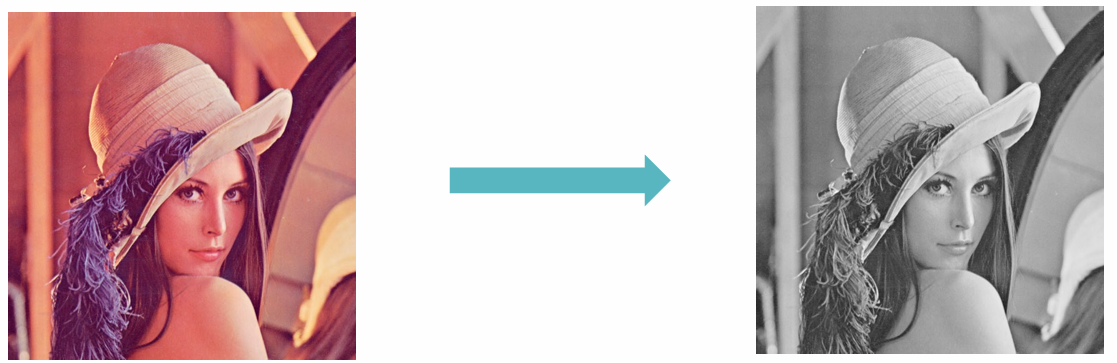
\includegraphics[width=0.7\textwidth]{figuresP/lesson_parallel_4_pag_19.png}
\end{center}

Assume you want to convert an image from RGB (where you have the colour code for each pixel) to greyscale. RGB is a standard to define the quantity of red, green, and blue in each pixel. A greyscale image is an image in which the value of each pixel carries only intensity information. For each pixel (I, J), the conversion formula is: $\text{grey\_Pixel}[I,J] = 0.21*r + 0.71*g + 0.07*b$. We multiply by floating point constants to perform the rescaling and store it. 

The following code contains the kernel i.e. the instructions that each thread must execute. In the main code there will be a part dedicated to copying the data from the host to the device and one that defines the number of threads that have to run the processing. Of course, since the small scheduler has limited dimensions, different multiprocessors might run different blocks, which in this case will correspond to different parts of the image. 

\begin{Verbatim}[label=\makebox{\url{https://github.com/lucabaldini/cmepda/tree/master/slides/latex/snippets/cuda_rgb_to_grayscale.cu}},commandchars=\\\{\}]
\PY{c+cp}{\#}\PY{c+cp}{define CHANNELS 3}

\PY{c+c1}{// GPU Kernel to convert RGB image to Grayscale}
\PY{k+kr}{\_\_global\_\_}\PY{+w}{ }\PY{k+kt}{void}\PY{+w}{ }\PY{n}{colorConvert}\PY{p}{(}\PY{k+kt}{unsigned}\PY{+w}{ }\PY{k+kt}{char}\PY{+w}{ }\PY{o}{*}\PY{+w}{ }\PY{n}{grayImage}\PY{p}{,}
\PY{+w}{                             }\PY{k+kt}{unsigned}\PY{+w}{ }\PY{k+kt}{char}\PY{+w}{ }\PY{o}{*}\PY{+w}{ }\PY{n}{rgbImage}\PY{p}{,}
\PY{+w}{                             }\PY{k+kt}{int}\PY{+w}{ }\PY{n}{width}\PY{p}{,}\PY{+w}{ }\PY{k+kt}{int}\PY{+w}{ }\PY{n}{height}\PY{p}{)}\PY{+w}{ }\PY{p}{\PYZob{}}

\PY{+w}{    }\PY{c+c1}{// Determine the (X, Y) pixel coordinates for this thread}
\PY{+w}{    }\PY{k+kt}{int}\PY{+w}{ }\PY{n}{x}\PY{+w}{ }\PY{o}{=}\PY{+w}{ }\PY{n+nb}{threadIdx}\PY{p}{.}\PY{n}{x}\PY{+w}{ }\PY{o}{+}\PY{+w}{ }\PY{n+nb}{blockIdx}\PY{p}{.}\PY{n}{x}\PY{+w}{ }\PY{o}{*}\PY{+w}{ }\PY{n+nb}{blockDim}\PY{p}{.}\PY{n}{x}\PY{p}{;}
\PY{+w}{    }\PY{k+kt}{int}\PY{+w}{ }\PY{n}{y}\PY{+w}{ }\PY{o}{=}\PY{+w}{ }\PY{n+nb}{threadIdx}\PY{p}{.}\PY{n}{y}\PY{+w}{ }\PY{o}{+}\PY{+w}{ }\PY{n+nb}{blockIdx}\PY{p}{.}\PY{n}{y}\PY{+w}{ }\PY{o}{*}\PY{+w}{ }\PY{n+nb}{blockDim}\PY{p}{.}\PY{n}{y}\PY{p}{;}

\PY{+w}{    }\PY{c+c1}{// Boundary check to prevent accessing memory outside the image}
\PY{+w}{    }\PY{k}{if}\PY{+w}{ }\PY{p}{(}\PY{n}{x}\PY{+w}{ }\PY{o}{\PYZlt{}}\PY{+w}{ }\PY{n}{width}\PY{+w}{ }\PY{o}{\PYZam{}}\PY{o}{\PYZam{}}\PY{+w}{ }\PY{n}{y}\PY{+w}{ }\PY{o}{\PYZlt{}}\PY{+w}{ }\PY{n}{height}\PY{p}{)}\PY{+w}{ }\PY{p}{\PYZob{}}

\PY{+w}{        }\PY{c+c1}{// Convert 2D coordinates to a 1D array index for the grayscale image}
\PY{+w}{        }\PY{k+kt}{int}\PY{+w}{ }\PY{n}{grayOffset}\PY{+w}{ }\PY{o}{=}\PY{+w}{ }\PY{n}{y}\PY{+w}{ }\PY{o}{*}\PY{+w}{ }\PY{n}{width}\PY{+w}{ }\PY{o}{+}\PY{+w}{ }\PY{n}{x}\PY{p}{;}

\PY{+w}{        }\PY{c+c1}{// Calculate the corresponding index in the RGB array (3 values per pixel)}
\PY{+w}{        }\PY{k+kt}{int}\PY{+w}{ }\PY{n}{rgbOffset}\PY{+w}{ }\PY{o}{=}\PY{+w}{ }\PY{n}{grayOffset}\PY{+w}{ }\PY{o}{*}\PY{+w}{ }\PY{n}{CHANNELS}\PY{p}{;}

\PY{+w}{        }\PY{c+c1}{// Extract Red, Green, and Blue channels (adjacent in memory)}
\PY{+w}{        }\PY{k+kt}{unsigned}\PY{+w}{ }\PY{k+kt}{char}\PY{+w}{ }\PY{n}{r}\PY{+w}{ }\PY{o}{=}\PY{+w}{ }\PY{n}{rgbImage}\PY{p}{[}\PY{n}{rgbOffset}\PY{+w}{    }\PY{p}{]}\PY{p}{;}
\PY{+w}{        }\PY{k+kt}{unsigned}\PY{+w}{ }\PY{k+kt}{char}\PY{+w}{ }\PY{n}{g}\PY{+w}{ }\PY{o}{=}\PY{+w}{ }\PY{n}{rgbImage}\PY{p}{[}\PY{n}{rgbOffset}\PY{+w}{ }\PY{o}{+}\PY{+w}{ }\PY{l+m+mi}{1}\PY{p}{]}\PY{p}{;}
\PY{+w}{        }\PY{k+kt}{unsigned}\PY{+w}{ }\PY{k+kt}{char}\PY{+w}{ }\PY{n}{b}\PY{+w}{ }\PY{o}{=}\PY{+w}{ }\PY{n}{rgbImage}\PY{p}{[}\PY{n}{rgbOffset}\PY{+w}{ }\PY{o}{+}\PY{+w}{ }\PY{l+m+mi}{2}\PY{p}{]}\PY{p}{;}

\PY{+w}{        }\PY{c+c1}{// Apply luminance formula to convert RGB to a single grayscale value}
\PY{+w}{        }\PY{n}{grayImage}\PY{p}{[}\PY{n}{grayOffset}\PY{p}{]}\PY{+w}{ }\PY{o}{=}\PY{+w}{ }\PY{p}{(}\PY{k+kt}{unsigned}\PY{+w}{ }\PY{k+kt}{char}\PY{p}{)}\PY{p}{(}\PY{l+m+mf}{0.21f}\PY{o}{*}\PY{n}{r}\PY{+w}{ }\PY{o}{+}\PY{+w}{ }\PY{l+m+mf}{0.71f}\PY{o}{*}\PY{n}{g}\PY{+w}{ }\PY{o}{+}\PY{+w}{ }\PY{l+m+mf}{0.07f}\PY{o}{*}\PY{n}{b}\PY{p}{)}\PY{p}{;}
\PY{+w}{    }\PY{p}{\PYZcb{}}
\PY{p}{\PYZcb{}}
\end{Verbatim}

\subsubsection{- GPUs and images: Blurring an image}
\begin{center}
    
\includegraphics[width=0.7\textwidth]{figuresP/lesson_parallel_4_pag_21.png}
\end{center}

Assume you want to blur an image. In this case, each thread defines a blurring box then the blurring comes from averaging the pixels in the box. Note that in these last 2 cases single threads execute operations on one pixel: there is not a 1 to 1 correspondence between pixels and single processors, but that is obviously not necessary. 

\begin{Verbatim}[label=\makebox{\url{https://github.com/lucabaldini/cmepda/tree/master/slides/latex/snippets/cuda_box_blur.cu}},commandchars=\\\{\}]
\PY{c+cp}{\#}\PY{c+cp}{define BLUR\_SIZE 1}

\PY{c+c1}{// GPU Kernel to apply a Box Blur filter to an image}
\PY{k+kr}{\_\_global\_\_}
\PY{k+kt}{void}\PY{+w}{ }\PY{n}{blurKernel}\PY{p}{(}\PY{k+kt}{unsigned}\PY{+w}{ }\PY{k+kt}{char}\PY{+w}{ }\PY{o}{*}\PY{+w}{ }\PY{n}{in}\PY{p}{,}\PY{+w}{ }\PY{k+kt}{unsigned}\PY{+w}{ }\PY{k+kt}{char}\PY{+w}{ }\PY{o}{*}\PY{+w}{ }\PY{n}{out}\PY{p}{,}\PY{+w}{ }\PY{k+kt}{int}\PY{+w}{ }\PY{n}{w}\PY{p}{,}\PY{+w}{ }\PY{k+kt}{int}\PY{+w}{ }\PY{n}{h}\PY{p}{)}\PY{+w}{ }\PY{p}{\PYZob{}}

\PY{+w}{    }\PY{c+c1}{// Determine the (X, Y) pixel coordinates for this thread}
\PY{+w}{    }\PY{k+kt}{int}\PY{+w}{ }\PY{n}{Col}\PY{+w}{ }\PY{o}{=}\PY{+w}{ }\PY{n+nb}{blockIdx}\PY{p}{.}\PY{n}{x}\PY{+w}{ }\PY{o}{*}\PY{+w}{ }\PY{n+nb}{blockDim}\PY{p}{.}\PY{n}{x}\PY{+w}{ }\PY{o}{+}\PY{+w}{ }\PY{n+nb}{threadIdx}\PY{p}{.}\PY{n}{x}\PY{p}{;}
\PY{+w}{    }\PY{k+kt}{int}\PY{+w}{ }\PY{n}{Row}\PY{+w}{ }\PY{o}{=}\PY{+w}{ }\PY{n+nb}{blockIdx}\PY{p}{.}\PY{n}{y}\PY{+w}{ }\PY{o}{*}\PY{+w}{ }\PY{n+nb}{blockDim}\PY{p}{.}\PY{n}{y}\PY{+w}{ }\PY{o}{+}\PY{+w}{ }\PY{n+nb}{threadIdx}\PY{p}{.}\PY{n}{y}\PY{p}{;}

\PY{+w}{    }\PY{c+c1}{// Boundary check for the main pixel}
\PY{+w}{    }\PY{k}{if}\PY{+w}{ }\PY{p}{(}\PY{n}{Col}\PY{+w}{ }\PY{o}{\PYZlt{}}\PY{+w}{ }\PY{n}{w}\PY{+w}{ }\PY{o}{\PYZam{}}\PY{o}{\PYZam{}}\PY{+w}{ }\PY{n}{Row}\PY{+w}{ }\PY{o}{\PYZlt{}}\PY{+w}{ }\PY{n}{h}\PY{p}{)}\PY{+w}{ }\PY{p}{\PYZob{}}
\PY{+w}{        }\PY{k+kt}{int}\PY{+w}{ }\PY{n}{pixVal}\PY{+w}{ }\PY{o}{=}\PY{+w}{ }\PY{l+m+mi}{0}\PY{p}{;}
\PY{+w}{        }\PY{k+kt}{int}\PY{+w}{ }\PY{n}{pixels}\PY{+w}{ }\PY{o}{=}\PY{+w}{ }\PY{l+m+mi}{0}\PY{p}{;}

\PY{+w}{        }\PY{c+c1}{// Loop over a local window/box centered around the current pixel}
\PY{+w}{        }\PY{k}{for}\PY{p}{(}\PY{k+kt}{int}\PY{+w}{ }\PY{n}{blurRow}\PY{+w}{ }\PY{o}{=}\PY{+w}{ }\PY{o}{\PYZhy{}}\PY{n}{BLUR\_SIZE}\PY{p}{;}\PY{+w}{ }\PY{n}{blurRow}\PY{+w}{ }\PY{o}{\PYZlt{}}\PY{+w}{ }\PY{n}{BLUR\_SIZE}\PY{o}{+}\PY{l+m+mi}{1}\PY{p}{;}\PY{+w}{ }\PY{o}{+}\PY{o}{+}\PY{n}{blurRow}\PY{p}{)}\PY{+w}{ }\PY{p}{\PYZob{}}
\PY{+w}{            }\PY{k}{for}\PY{p}{(}\PY{k+kt}{int}\PY{+w}{ }\PY{n}{blurCol}\PY{+w}{ }\PY{o}{=}\PY{+w}{ }\PY{o}{\PYZhy{}}\PY{n}{BLUR\_SIZE}\PY{p}{;}\PY{+w}{ }\PY{n}{blurCol}\PY{+w}{ }\PY{o}{\PYZlt{}}\PY{+w}{ }\PY{n}{BLUR\_SIZE}\PY{o}{+}\PY{l+m+mi}{1}\PY{p}{;}\PY{+w}{ }\PY{o}{+}\PY{o}{+}\PY{n}{blurCol}\PY{p}{)}\PY{+w}{ }\PY{p}{\PYZob{}}

\PY{+w}{                }\PY{c+c1}{// Calculate coordinates of the neighbor pixel}
\PY{+w}{                }\PY{k+kt}{int}\PY{+w}{ }\PY{n}{curRow}\PY{+w}{ }\PY{o}{=}\PY{+w}{ }\PY{n}{Row}\PY{+w}{ }\PY{o}{+}\PY{+w}{ }\PY{n}{blurRow}\PY{p}{;}
\PY{+w}{                }\PY{k+kt}{int}\PY{+w}{ }\PY{n}{curCol}\PY{+w}{ }\PY{o}{=}\PY{+w}{ }\PY{n}{Col}\PY{+w}{ }\PY{o}{+}\PY{+w}{ }\PY{n}{blurCol}\PY{p}{;}

\PY{+w}{                }\PY{c+c1}{// Check if the neighbor pixel is actually inside image boundaries}
\PY{+w}{                }\PY{k}{if}\PY{p}{(}\PY{n}{curRow}\PY{+w}{ }\PY{o}{\PYZgt{}}\PY{+w}{ }\PY{l+m+mi}{\PYZhy{}1}\PY{+w}{ }\PY{o}{\PYZam{}}\PY{o}{\PYZam{}}\PY{+w}{ }\PY{n}{curRow}\PY{+w}{ }\PY{o}{\PYZlt{}}\PY{+w}{ }\PY{n}{h}\PY{+w}{ }\PY{o}{\PYZam{}}\PY{o}{\PYZam{}}\PY{+w}{ }\PY{n}{curCol}\PY{+w}{ }\PY{o}{\PYZgt{}}\PY{+w}{ }\PY{l+m+mi}{\PYZhy{}1}\PY{+w}{ }\PY{o}{\PYZam{}}\PY{o}{\PYZam{}}\PY{+w}{ }\PY{n}{curCol}\PY{+w}{ }\PY{o}{\PYZlt{}}\PY{+w}{ }\PY{n}{w}\PY{p}{)}\PY{+w}{ }\PY{p}{\PYZob{}}

\PY{+w}{                    }\PY{c+c1}{// Accumulate neighbor pixel values}
\PY{+w}{                    }\PY{n}{pixVal}\PY{+w}{ }\PY{o}{+}\PY{o}{=}\PY{+w}{ }\PY{n}{in}\PY{p}{[}\PY{n}{curRow}\PY{+w}{ }\PY{o}{*}\PY{+w}{ }\PY{n}{w}\PY{+w}{ }\PY{o}{+}\PY{+w}{ }\PY{n}{curCol}\PY{p}{]}\PY{p}{;}
\PY{+w}{                    }\PY{c+c1}{// Count valid neighbors to compute the average later}
\PY{+w}{                    }\PY{n}{pixels}\PY{o}{+}\PY{o}{+}\PY{p}{;}
\PY{+w}{                }\PY{p}{\PYZcb{}}
\PY{+w}{            }\PY{p}{\PYZcb{}}
\PY{+w}{        }\PY{p}{\PYZcb{}}
\PY{+w}{        }\PY{c+c1}{// Compute the average (blur) and write it to the output image array}
\PY{+w}{        }\PY{n}{out}\PY{p}{[}\PY{n}{Row}\PY{+w}{ }\PY{o}{*}\PY{+w}{ }\PY{n}{w}\PY{+w}{ }\PY{o}{+}\PY{+w}{ }\PY{n}{Col}\PY{p}{]}\PY{+w}{ }\PY{o}{=}\PY{+w}{ }\PY{p}{(}\PY{k+kt}{unsigned}\PY{+w}{ }\PY{k+kt}{char}\PY{p}{)}\PY{p}{(}\PY{n}{pixVal}\PY{+w}{ }\PY{o}{/}\PY{+w}{ }\PY{n}{pixels}\PY{p}{)}\PY{p}{;}
\PY{+w}{    }\PY{p}{\PYZcb{}}
\PY{p}{\PYZcb{}}
\end{Verbatim}

\subsection{CUDA program structure}
From the previous examples, you should have understood the typical structure of a CUDA program:
\begin{itemize}
    \item \textbf{Global Declarations:} Declaration of global variables and device functions.
    \item \textbf{Host Code (\texttt{main()}):} The CPU control flow, which typically involves:
    \begin{itemize}
        \item Allocating memory space on the device (GPU).
        \item Transferring data from the host (CPU) to the device.
        \item Setting up the execution configuration (defining grid and block dimensions).
        \item Calling the kernel (e.g., \texttt{kernelOne<<<grid, block>>>(args...)}).
        \item Transferring the computed results from the device back to the host.
        \item Optionally verifying the output against a golden (host-computed) solution.
    \end{itemize}
    \item \textbf{Device Code (\texttt{\_\_global\_\_ void kernelOne(...)}):} The kernel function executed in parallel on the GPU. It includes the declaration of local and shared variables (automatic variables are transparently assigned to registers or local memory) and the use of \texttt{\_\_syncthreads()} for block-level thread synchronization.
\end{itemize}

\hrulefill

\subsection{Note: Evolution of PC Architectures, from Shared Buses to PCIe}

In older PC architectures, system communication relied on a shared bus system managed by two main chips. The Northbridge connected the three components that required high-speed communication: the CPU, the DRAM, and the video card, ensuring the latter had 1st-class access to the main memory. For instance, older NVIDIA cards connected via the AGP bus, achieving transfer rates of up to 2 GB/s. Conversely, the Southbridge acted as a concentrator for slower I/O devices, such as the ATA Bus. The traditional PCI bus, which was connected to the Southbridge, was initially a shared 33 MHz, 32-bit wide bus with a 132 MB/s peak transfer rate, later evolving to 66 MHz and 64-bit to reach a 528 MB/s peak. However, due to its shared nature and the need for bus arbitration, the upstream bandwidth remained a bottleneck for devices, peaking at around 256 MB/s.

\begin{center}
    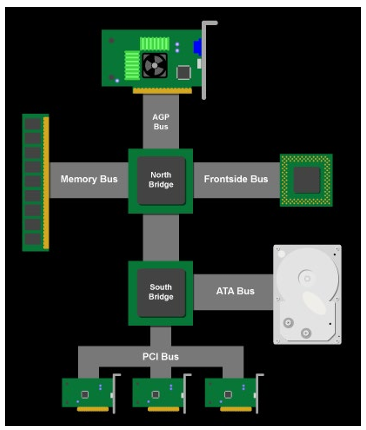
\includegraphics[width=0.4\textwidth]{figuresP/lesson_parallel_4_pag_24.png}
\end{center}

To overcome these limitations, PCI Express (PCIe) was introduced, replacing the shared bus with switched point-to-point serial links across multiple lanes. Because each card now has a dedicated link to a central switch, bus arbitration is completely eliminated. A single PCIe lane is 1-bit wide and consists of 4 wires. In PCIe Gen3, each 2-wire pair can transmit 8 Gb/s in one direction, allowing for simultaneous and symmetric upstream and downstream communication. To maintain signal integrity, data relies on an 8b/10b encoding scheme (where each byte of data is encoded into 10 bits with an equal number of 1's and 0's), yielding a net data rate of approximately 2 Gb/s per lane, each way. By combining multiple lanes into a single link (x1, x2, x4, x8, x12, or x16), bandwidth scales accordingly. Consequently, the net data rates translate to roughly 985 MB/s (x1), 2 GB/s (x2), and 4 GB/s (x4) in each direction.

\begin{center}
    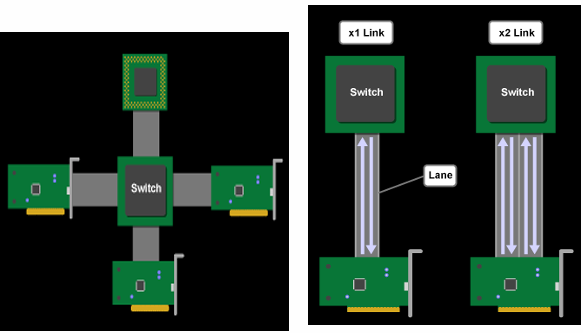
\includegraphics[width=0.8\textwidth]{figuresP/lesson_parallel_4_pag_25.png}
\end{center}

This shift to PCIe significantly altered the overall PC architecture. While earlier systems (up to PCIe Gen2) simply repurposed the North Bridge and South Bridge as PCIe switches, modern architectures integrate both bridges directly into the main processor. Today, while PCIe remains the standard, other specialized fast buses, such as NVLINK, serve as high-performance alternatives for demanding workloads.

\begin{center}
    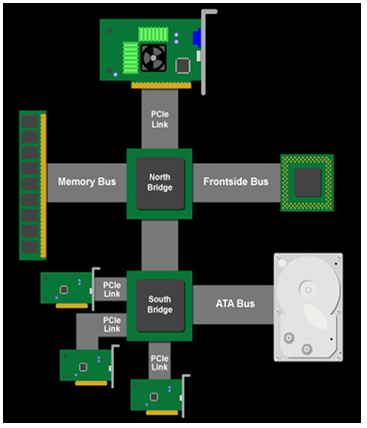
\includegraphics[width=0.4\textwidth]{figuresP/lesson_parallel_4_pag_26.png}
\end{center}

\hrulefill

\begin{minipage}[c]{0.6\textwidth}
    \subsection{The bandwidth problem}
    The bandwidth (and the latency) of the \textit{data transfer between host and device is the main bottleneck of GPU computing} (and also between GPU processor and global memory). This is especially true for massively parallel systems processing massive amounts of data. Tricks like buffering, reordering, and caching can temporarily defy the rules in some cases and modern GPUs will have faster and faster PCIe. Streaming data transfer and processing is a winning strategy to hide latency. Hardware strategies (like DMA, Direct Memory Access) are used to mitigate the data transfer problem, but the concept remains valid: the GPU is made mainly for computation.\\
    That's another aspect you should think about when you are deciding whether to use GPUs or not: if your program needs to access the memory many times, maybe you should actually use a sequential set of instructions. However, if you need to execute a lot of simple instruction on the same set of data, that's when GPUs really shine.
\end{minipage}\hfill 
\begin{minipage}[c]{0.35\textwidth}
    \centering
    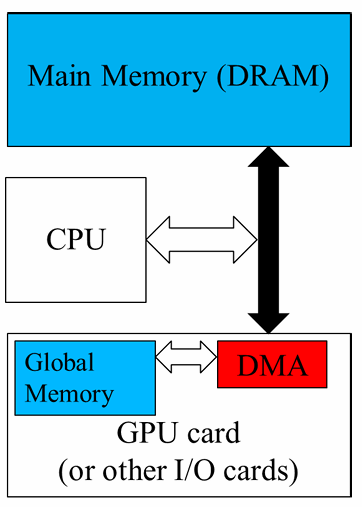
\includegraphics[width=\textwidth]{figuresP/lesson_parallel_4_pag_27.png}
\end{minipage}

\newpage

\section{Hands-on examples for parallel programming}\label{sec:hands_on_cuda_1}
With all that has been said in the last two sections, you may feel overwhelmed by all of these new concepts and methods of GPU programming. Fortunately for you, these last sections of the chapter are all about hands-on examples for parallel programming. As always, feel free to write your own code and experiment with it for as long as you can to become familiar with GPUs.

In the following table, you can find the specifics of the GPU used during the 2025-26 classes.

\begin{center}
    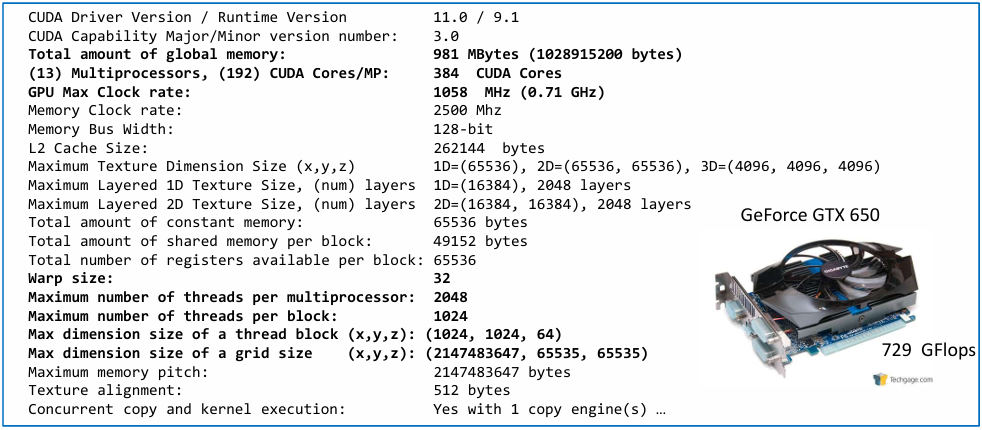
\includegraphics[width=0.9\textwidth]{figuresP/lesson_parallel_4_pag_29.png}
\end{center}

However, I will be using the NVIDIA GeForce MX330 GPU inside my PC to run and modify the code. Its specs are listed in the table below.

\begin{table*}[htbp]
    \centering
    \small
    \begin{tabular}{|ll|}
    \hline
        CUDA Capability Major/Minor version number: & 6.1 \\
        Total amount of global memory: & 2048 MBytes (2147483648 bytes) \\
        (3) Multiprocessors, (128) CUDA Cores/MP: & 384 CUDA Cores \\
        GPU Max Clock rate: & 1594 MHz (1.59 GHz) \\
        Theoretical Peak Performance (FP32): & 1.22 TeraFLOPS \\
        Memory Clock rate: & 3504 MHz \\
        Memory Bus Width: & 64-bit \\
        L2 Cache Size: & 524288 bytes \\
        Total amount of constant memory: & 65536 bytes \\
        Total amount of shared memory per block: & 49152 bytes \\
        Total number of registers available per block: & 65536 \\
        Warp size: & 32 \\
        Maximum number of threads per multiprocessor: & 2048 \\
        Maximum number of threads per block: & 1024 \\
        Max dimension size of a thread block (x,y,z): & (1024, 1024, 64) \\
        Max dimension size of a grid size (x,y,z): & (2147483647, 65535, 65535) \\
        Texture alignment: & 512 bytes \\
        Concurrent copy and kernel execution: & Yes with 1 copy engine(s) \\
    \hline
    \end{tabular}
\end{table*}

In order to try and run the following examples at home, you must have an NVIDIA GPU attached to your PC. If you do have it, then you just need to install the CUDA Toolkit and have fun. Pay attention: you should always check which version of the CUDA Toolkit is compatible with your GPU before installing. However, if you don't have an NVIDIA GPU you can use online resources like Google Colab that let you use a graphics processing unit directly from their platform. 

\subsection{"Hello World!" with Cuda}

Here is our first example of a piece of code running on the GPU:

\begin{Verbatim}[label=\makebox{\url{https://github.com/lucabaldini/cmepda/tree/master/slides/latex/snippets/cuda_hello_world.cu}},commandchars=\\\{\}]
\PY{c+cp}{\#}\PY{c+cp}{include}\PY{+w}{ }\PY{c+cpf}{\PYZlt{}cuda.h\PYZgt{}}
\PY{c+cp}{\#}\PY{c+cp}{include}\PY{+w}{ }\PY{c+cpf}{\PYZlt{}stdio.h\PYZgt{}}

\PY{c+c1}{// The word \PYZdq{}\_\_global\_\_\PYZdq{} is not C standard! You need \#include \PYZlt{}cuda.h\PYZgt{} !}

\PY{c+c1}{// Part of the code running on the GPU: the kernel (with no arguments and no returns)}
\PY{k+kr}{\_\_global\_\_}\PY{+w}{ }\PY{k+kt}{void}\PY{+w}{ }\PY{n}{mykernel}\PY{p}{(}\PY{k+kt}{void}\PY{p}{)}\PY{+w}{ }\PY{p}{\PYZob{}}
\PY{+w}{  }\PY{n}{printf}\PY{p}{(}\PY{l+s}{\PYZdq{}}\PY{l+s}{Hello World from GPU! (block: \PYZpc{}d thread: \PYZpc{}d)}\PY{l+s+se}{\PYZbs{}n}\PY{l+s}{\PYZdq{}}\PY{p}{,}\PY{n+nb}{blockIdx}\PY{p}{.}\PY{n}{x}\PY{p}{,}\PY{n+nb}{threadIdx}\PY{p}{.}\PY{n}{x}\PY{p}{)}\PY{p}{;}
\PY{p}{\PYZcb{}}

\PY{c+c1}{// Part of the code running on the CPU}
\PY{k+kt}{int}\PY{+w}{ }\PY{n}{main}\PY{p}{(}\PY{k+kt}{void}\PY{p}{)}\PY{+w}{ }\PY{p}{\PYZob{}}
\PY{+w}{  }\PY{c+c1}{// I\PYZsq{}m using 5 blocks with 2 threads per block to run the kernel}
\PY{+w}{  }\PY{n}{mykernel}\PY{+w}{ }\PY{o}{\PYZlt{}}\PY{o}{\PYZlt{}}\PY{o}{\PYZlt{}}\PY{l+m+mi}{5}\PY{p}{,}\PY{l+m+mi}{2}\PY{o}{\PYZgt{}}\PY{o}{\PYZgt{}}\PY{o}{\PYZgt{}}\PY{p}{(}\PY{p}{)}\PY{p}{;}
\PY{+w}{  }\PY{n}{cudaDeviceSynchronize}\PY{p}{(}\PY{p}{)}\PY{p}{;}
\PY{+w}{  }\PY{n}{printf}\PY{p}{(}\PY{l+s}{\PYZdq{}}\PY{l+s}{Hello World from Host!}\PY{l+s+se}{\PYZbs{}n}\PY{l+s}{\PYZdq{}}\PY{p}{)}\PY{p}{;}
\PY{+w}{  }\PY{k}{return}\PY{+w}{ }\PY{l+m+mi}{0}\PY{p}{;}
\PY{p}{\PYZcb{}}

[Output]
Hello World from GPU! (block: 3 thread: 0)                                                                      
Hello World from GPU! (block: 3 thread: 1)
Hello World from GPU! (block: 0 thread: 0)
Hello World from GPU! (block: 0 thread: 1)
Hello World from GPU! (block: 4 thread: 0)
Hello World from GPU! (block: 4 thread: 1)
Hello World from GPU! (block: 1 thread: 0)
Hello World from GPU! (block: 1 thread: 1)
Hello World from GPU! (block: 2 thread: 0)
Hello World from GPU! (block: 2 thread: 1)
Hello World from Host!
\end{Verbatim}

As you can see, this is very similar to a standard C code. You have your \texttt{main} function and your standard \texttt{\#include <stdio.h>} that lets you use your \texttt{printf} function. \\ However, the term \texttt{\_\_global\_\_} is not C standard and is imported using \texttt{\#include <cuda.h>}. The \texttt{\_\_global\_\_} execution space specifier tells the compiler that this is a \textit{kernel} function which, as we said before, is a function executed on the GPU but called from the host. In this case, it has no parameters and no returns, as specified by the use of \texttt{void}. \\ 
The command \texttt{cudaDeviceSynchronize()} is crucial. In CUDA, kernel launches are \textit{asynchronous}: the CPU issues the command to start the kernel and immediately moves to the next instruction without waiting for the GPU. \\
\texttt{blockIdx.x} and \texttt{threadIdx.x} identify the block and the thread that are running the code, as you can see in the return. \\
\texttt{cudaDeviceSynchronize()} forces the CPU to halt and wait until all GPU tasks are completely finished, ensuring the GPU's print statements are processed before the program ends. Try and comment this line to see what happens.

Now, how do we run this? First of all, you need to compile it using the CUDA compiler called \textbf{NVCC}, which will be automatically installed with the Toolkit. On Windows you must run \\
\texttt{nvcc HelloWorldGpu.cu -o HelloWorldGpu.exe} \\ 
\footnote{Depending on your GPU's physical architecture and your CUDA Toolkit version, you might need to specify the target architecture during compilation using the \texttt{-arch} flag (e.g., \texttt{-arch=sm\_61} for Pascal-based GPUs like the MX330 or GTX 10-series). This is because newer versions of the CUDA compiler periodically drop support for older GPU architectures. If you encounter an "Unsupported gpu architecture" error, you will need to either append this flag or install an older, compatible version of the Toolkit.} 
(you can input whatever name you want for the executable file after the \texttt{-o}) and then \\
\texttt{.\textbackslash HelloWorldGpu.exe} \\
to actually execute the code. On Linux it is all very similar: \\
\texttt{nvcc HelloWorldGpu.cu -o HelloWorldGpu} \\
\texttt{./HelloWorldGpu}

Note that it is not always true that block 0 is executed before block 1 and so on: the big scheduler can organize the execution in a way that can appear non sequential (Of course! It's parallel computing!). In our case, the "strange" output is due to the fact that we asked the GPU to run 5 blocks of code when it only contains 3 multiprocessors \footnote{That is not actually true for our simple \texttt{printf} function, but let's pretend}. The same thing could happen with threads, and the effect could have been clear if I had written a code with more than 128 threads per block. You can actually force the GPU to execute blocks and threads in a precise order, but that will probably slow down your execution. 

\subsection{Vector sum: CUDA vs. C}
Take a look at the following example. It is a simple serial code that runs entirely on the CPU (CUDA is used exclusively to measure the execution time). Here's what it does in detail:

\begin{itemize}
    \item[-] The \texttt{RandomVector} function (lines 6-10) initializes an array with random integers between 1 and 100. 
    
    \item[-] The \texttt{VecAddSerial} (lines 13-17) function performs a standard element-by-element vector addition on the CPU using a simple \texttt{for} loop.
    
    \item[-] Inside the \texttt{main} function, standard C \texttt{malloc} (lines 29-31) is used to allocate memory on the host (CPU) for three large vectors of size $N = 1048576$ elements.
    
    \item[-] The program leverages the CUDA to measure the elapsed time. It declares two events of type \texttt{cudaEvent\_t} (\texttt{start} and \texttt{stop}) and creates them using \texttt{cudaEventCreate} (lines 24-26).
    
    \item[-] \texttt{cudaEventRecord(start)} marks the beginning of the timer then \texttt{VecAddSerial(h\_a, h\_b, h\_c)} executes the addition entirely on the CPU and \texttt{cudaEventRecord(stop)} marks the end of the operation (lines 36-43).
    
    \item[-] \texttt{cudaEventSynchronize(stop)} (line 43) is called to ensure that all operations associated with the \texttt{stop} event are fully completed before proceeding. 
    
    \item[-] \texttt{cudaEventElapsedTime} (line 44) calculates the time difference between the events in ms. 
    
    \item[-] Finally, the result is printed to the console\footnote{In reality the output will change every time you execute the code, but not by much. The output below is a reference value, and so will be the time measures in the next examples.}, and the host memory is released using \texttt{free()} (lines 47-52).
\end{itemize}

\begin{Verbatim}[label=\makebox{\url{https://github.com/lucabaldini/cmepda/tree/master/slides/latex/snippets/cuda_vec_add_serial.cu}},commandchars=\\\{\}]
\PY{c+cp}{\#}\PY{c+cp}{include}\PY{+w}{ }\PY{c+cpf}{\PYZlt{}stdio.h\PYZgt{}}
\PY{c+cp}{\#}\PY{c+cp}{include}\PY{+w}{ }\PY{c+cpf}{\PYZlt{}stdlib.h\PYZgt{}}\PY{c+c1}{ // Added for rand() and malloc()}
\PY{c+cp}{\#}\PY{c+cp}{define N 1048576}

\PY{c+c1}{// Function to define a vector with N elements (with N\PYZgt{}10\PYZca{}6)}
\PY{k+kt}{void}\PY{+w}{ }\PY{n+nf}{RandomVector}\PY{p}{(}\PY{k+kt}{int}\PY{+w}{ }\PY{o}{*}\PY{n}{a}\PY{p}{,}\PY{+w}{ }\PY{k+kt}{int}\PY{+w}{ }\PY{n}{nn}\PY{p}{)}\PY{p}{\PYZob{}}
\PY{+w}{  }\PY{k}{for}\PY{+w}{ }\PY{p}{(}\PY{k+kt}{int}\PY{+w}{ }\PY{n}{i}\PY{o}{=}\PY{l+m+mi}{0}\PY{p}{;}\PY{n}{i}\PY{o}{\PYZlt{}}\PY{n}{nn}\PY{p}{;}\PY{n}{i}\PY{o}{+}\PY{o}{+}\PY{p}{)}\PY{+w}{ }\PY{p}{\PYZob{}}
\PY{+w}{    }\PY{n}{a}\PY{p}{[}\PY{n}{i}\PY{p}{]}\PY{o}{=}\PY{n}{rand}\PY{p}{(}\PY{p}{)}\PY{o}{\PYZpc{}}\PY{l+m+mi}{100}\PY{o}{+}\PY{l+m+mi}{1}\PY{p}{;}
\PY{+w}{  }\PY{p}{\PYZcb{}}
\PY{p}{\PYZcb{}}

\PY{c+c1}{// Function to add 2 vectors using a for cycle}
\PY{k+kt}{void}\PY{+w}{ }\PY{n+nf}{VecAddSerial}\PY{p}{(}\PY{k+kt}{int}\PY{+w}{ }\PY{o}{*}\PY{n}{a}\PY{p}{,}\PY{+w}{ }\PY{k+kt}{int}\PY{+w}{ }\PY{o}{*}\PY{n}{b}\PY{p}{,}\PY{+w}{ }\PY{k+kt}{int}\PY{+w}{ }\PY{o}{*}\PY{n}{c}\PY{p}{)}\PY{p}{\PYZob{}}
\PY{+w}{  }\PY{k}{for}\PY{+w}{ }\PY{p}{(}\PY{k+kt}{int}\PY{+w}{ }\PY{n}{i}\PY{o}{=}\PY{l+m+mi}{0}\PY{p}{;}\PY{n}{i}\PY{o}{\PYZlt{}}\PY{n}{N}\PY{p}{;}\PY{n}{i}\PY{o}{+}\PY{o}{+}\PY{p}{)}\PY{p}{\PYZob{}}
\PY{+w}{    }\PY{n}{c}\PY{p}{[}\PY{n}{i}\PY{p}{]}\PY{+w}{ }\PY{o}{=}\PY{+w}{ }\PY{n}{a}\PY{p}{[}\PY{n}{i}\PY{p}{]}\PY{o}{+}\PY{n}{b}\PY{p}{[}\PY{n}{i}\PY{p}{]}\PY{p}{;}
\PY{+w}{  }\PY{p}{\PYZcb{}}
\PY{p}{\PYZcb{}}

\PY{k+kt}{int}\PY{+w}{ }\PY{n+nf}{main}\PY{p}{(}\PY{k+kt}{void}\PY{p}{)}\PY{+w}{ }\PY{p}{\PYZob{}}
\PY{+w}{  }\PY{k+kt}{int}\PY{+w}{ }\PY{o}{*}\PY{n}{h\_a}\PY{p}{,}\PY{+w}{ }\PY{o}{*}\PY{n}{h\_b}\PY{p}{,}\PY{+w}{ }\PY{o}{*}\PY{n}{h\_c}\PY{p}{;}
\PY{+w}{  }\PY{k+kt}{int}\PY{+w}{ }\PY{n}{size}\PY{+w}{ }\PY{o}{=}\PY{+w}{ }\PY{n}{N}\PY{o}{*}\PY{k}{sizeof}\PY{p}{(}\PY{k+kt}{int}\PY{p}{)}\PY{p}{;}

\PY{+w}{  }\PY{k+kt}{float}\PY{+w}{ }\PY{n}{time}\PY{p}{;}
\PY{+w}{  }\PY{n}{cudaEvent\_t}\PY{+w}{ }\PY{n}{start}\PY{p}{,}\PY{n}{stop}\PY{p}{;}
\PY{+w}{  }\PY{n}{cudaEventCreate}\PY{p}{(}\PY{o}{\PYZam{}}\PY{n}{start}\PY{p}{)}\PY{p}{;}
\PY{+w}{  }\PY{n}{cudaEventCreate}\PY{p}{(}\PY{o}{\PYZam{}}\PY{n}{stop}\PY{p}{)}\PY{p}{;}

\PY{+w}{  }\PY{c+c1}{// Allocation of a memory space in the host for the 2 vectors (and filling)}
\PY{+w}{  }\PY{n}{h\_a}\PY{+w}{ }\PY{o}{=}\PY{+w}{ }\PY{p}{(}\PY{k+kt}{int}\PY{+w}{ }\PY{o}{*}\PY{p}{)}\PY{n}{malloc}\PY{p}{(}\PY{n}{size}\PY{p}{)}\PY{p}{;}
\PY{+w}{  }\PY{n}{h\_b}\PY{+w}{ }\PY{o}{=}\PY{+w}{ }\PY{p}{(}\PY{k+kt}{int}\PY{+w}{ }\PY{o}{*}\PY{p}{)}\PY{n}{malloc}\PY{p}{(}\PY{n}{size}\PY{p}{)}\PY{p}{;}
\PY{+w}{  }\PY{n}{h\_c}\PY{+w}{ }\PY{o}{=}\PY{+w}{ }\PY{p}{(}\PY{k+kt}{int}\PY{+w}{ }\PY{o}{*}\PY{p}{)}\PY{n}{malloc}\PY{p}{(}\PY{n}{size}\PY{p}{)}\PY{p}{;}
\PY{+w}{  }\PY{n}{RandomVector}\PY{p}{(}\PY{n}{h\_a}\PY{p}{,}\PY{n}{N}\PY{p}{)}\PY{p}{;}
\PY{+w}{  }\PY{n}{RandomVector}\PY{p}{(}\PY{n}{h\_b}\PY{p}{,}\PY{n}{N}\PY{p}{)}\PY{p}{;}

\PY{+w}{  }\PY{c+c1}{// Start time}
\PY{+w}{  }\PY{n}{cudaEventRecord}\PY{p}{(}\PY{n}{start}\PY{p}{)}\PY{p}{;}

\PY{+w}{  }\PY{c+c1}{//Launch serial sum on CPU}
\PY{+w}{  }\PY{n}{VecAddSerial}\PY{p}{(}\PY{n}{h\_a}\PY{p}{,}\PY{n}{h\_b}\PY{p}{,}\PY{n}{h\_c}\PY{p}{)}\PY{p}{;}

\PY{+w}{  }\PY{c+c1}{// Stop time}
\PY{+w}{  }\PY{n}{cudaEventRecord}\PY{p}{(}\PY{n}{stop}\PY{p}{)}\PY{p}{;}
\PY{+w}{  }\PY{n}{cudaEventSynchronize}\PY{p}{(}\PY{n}{stop}\PY{p}{)}\PY{p}{;}
\PY{+w}{  }\PY{n}{cudaEventElapsedTime}\PY{p}{(}\PY{o}{\PYZam{}}\PY{n}{time}\PY{p}{,}\PY{+w}{ }\PY{n}{start}\PY{p}{,}\PY{+w}{ }\PY{n}{stop}\PY{p}{)}\PY{p}{;}

\PY{+w}{  }\PY{c+c1}{// Print time}
\PY{+w}{  }\PY{n}{printf}\PY{p}{(}\PY{l+s}{\PYZdq{}}\PY{l+s}{Time: \PYZpc{}3.5f ms}\PY{l+s+se}{\PYZbs{}n}\PY{l+s}{\PYZdq{}}\PY{p}{,}\PY{n}{time}\PY{p}{)}\PY{p}{;}

\PY{+w}{  }\PY{c+c1}{// Cleanup}
\PY{+w}{  }\PY{n}{free}\PY{p}{(}\PY{n}{h\_a}\PY{p}{)}\PY{p}{;}
\PY{+w}{  }\PY{n}{free}\PY{p}{(}\PY{n}{h\_b}\PY{p}{)}\PY{p}{;}
\PY{+w}{  }\PY{n}{free}\PY{p}{(}\PY{n}{h\_c}\PY{p}{)}\PY{p}{;}

\PY{+w}{  }\PY{k}{return}\PY{p}{(}\PY{l+m+mi}{0}\PY{p}{)}\PY{p}{;}
\PY{p}{\PYZcb{}}

[Output]
Time: 4.34893 ms
\end{Verbatim}

Now we should try and parallelize our computation. At first glance this next example seems to do just that. \\ The \texttt{VecAddGpu} kernel (lines 13-15) is executed by the GPU and it should speed up the process. Note that in order to use the kernel, the program copies the vectors defined in the host memory (\texttt{h\_a}, \texttt{h\_b}, \texttt{h\_c}) to the device memory (\texttt{d\_a}, \texttt{d\_b}, \texttt{d\_c}) using \texttt{cudaMalloc} and \texttt{cudaMemcpy} (lines 35-41). Also, it copies the result of the computation back to the host (line 56).

\input{pygments/Cuda_VecAdd_Blocks}

\begin{figure}[htbp]
    \begin{minipage}[c]{0.55\textwidth}
    Now, if you take a look at the output, it surely isn't optimal: the execution time has more than doubled. As said, the act of moving data from host to device and vice versa might slow down our execution, but in this case the problem is elsewhere, and once you notice it, it is pretty obvious. 
    \newline\newline Take a look at line 48:\\
    \texttt{VecAddGpu<<<1,N>>>(d\_a,d\_b,d\_c);} \\
    It is saying that we are running more than a million blocks with a single thread per block (as represented in figure)! Each of the 3 multiprocessors in our GPU is running a block, but only one of its cores (which is slower than the CPU),is actually working, while the other 127 are doing nothing! That is not parallelization, it is a waste of computing power.
    \end{minipage}\hfill 
    \begin{minipage}[c]{0.4\textwidth}
        \centering
        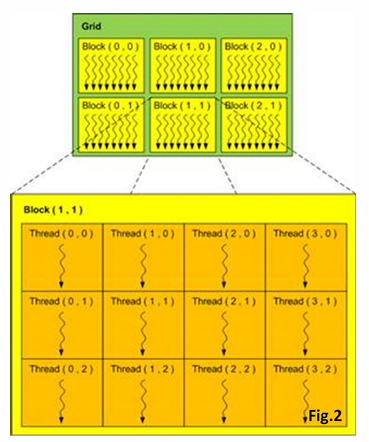
\includegraphics[width=\textwidth]{figuresP/lesson_parallel_4_pag_33.png}
    \end{minipage}
\end{figure} 

We could also ask ourselves what would happen if instead we tried to divide the computation in a million threads inside the same block. That's fairly easy to implement: just rewrite the kernel (lines 13-15) as such
\begin{Verbatim}[commandchars=\\\{\}]
\PY{k+kr}{\_\_global\_\_}\PY{+w}{ }\PY{k+kt}{void}\PY{+w}{ }\PY{n}{VecAddGpu}\PY{p}{(}\PY{k+kt}{int}\PY{+w}{ }\PY{o}{*}\PY{n}{a}\PY{p}{,}\PY{+w}{ }\PY{k+kt}{int}\PY{+w}{ }\PY{o}{*}\PY{n}{b}\PY{p}{,}\PY{+w}{ }\PY{k+kt}{int}\PY{+w}{ }\PY{o}{*}\PY{n}{c}\PY{p}{)}\PY{p}{\PYZob{}}
\PY{+w}{  }\PY{n}{c}\PY{p}{[}\PY{n+nb}{threadIdx}\PY{p}{.}\PY{n}{x}\PY{p}{]}\PY{+w}{ }\PY{o}{=}\PY{+w}{ }\PY{n}{a}\PY{p}{[}\PY{n+nb}{threadIdx}\PY{p}{.}\PY{n}{x}\PY{p}{]}\PY{o}{+}\PY{n}{b}\PY{p}{[}\PY{n+nb}{threadIdx}\PY{p}{.}\PY{n}{x}\PY{p}{]}\PY{p}{;}
\PY{p}{\PYZcb{}}
\end{Verbatim}
and launch it with (line 47)
\begin{Verbatim}[commandchars=\\\{\}]
\PY{n}{VecAddGpu}\PY{o}{\PYZlt{}}\PY{o}{\PYZlt{}}\PY{o}{\PYZlt{}}\PY{l+m+mi}{1}\PY{p}{,}\PY{n}{N}\PY{o}{\PYZgt{}}\PY{o}{\PYZgt{}}\PY{o}{\PYZgt{}}\PY{p}{(}\PY{n}{d\_a}\PY{p}{,}\PY{n}{d\_b}\PY{p}{,}\PY{n}{d\_c}\PY{p}{)}\PY{p}{;}
\end{Verbatim}
In my own device the output is \texttt{Time: 0.15997 ms}. That seems wonderful, a speed-up of about 40 with respect to the serial code. However, something is wrong and you can check it in 2 ways:
\begin{itemize}
\item[-] Try to print your result (maybe not all the million or so elements of \texttt{h\_c}, but the first 2 or 3 hundred): you will find that they are all equal to zero. 
\item[-] After the stop time instruction, "ask" CUDA if an error was found (this is the best practice) using 
\begin{Verbatim}[commandchars=\\\{\}]
\PY{n}{cudaError\_t}\PY{+w}{ }\PY{n}{KernelError}\PY{+w}{ }\PY{o}{=}\PY{+w}{ }\PY{n}{cudaGetLastError}\PY{p}{(}\PY{p}{)}\PY{p}{;}
\PY{n}{printf}\PY{p}{(}\PY{l+s}{\PYZdq{}}\PY{l+s}{Error: \PYZpc{}s}\PY{l+s+se}{\PYZbs{}n}\PY{l+s}{\PYZdq{}}\PY{p}{,}\PY{+w}{ }\PY{n}{cudaGetErrorString}\PY{p}{(}\PY{n}{KernelError}\PY{p}{)}\PY{p}{)}\PY{p}{;}
\end{Verbatim}
Your output should read \texttt{Error: invalid configuration argument}.
\end{itemize}
Go back to the specifics of our GPU: the maximum number of threads per block is 1024, which is way lower with respect to the million elements of the vector. Our device cannot execute our instructions! 

That should teach you an important lesson: \textbf{a serial code is much more portable than a parallel one}. In other words, the way you run your programs is much more dependent on the machine you are running them on if you are using the GPU instead of the simple CPU. Before starting to work on the device instead of the host, you must always be aware of its characteristics. 

Now no more tricks: down here you will find how you should really write this code in order to make it parallel. \\Note that we are using 128 threads per block. Even if the maximum number of threads per block is 1024, we know that our GPU has 128 cores per multiprocessor. For this reason, in this kind of operation, we won't have a significant speed up using a number of threads higher than 128. \\ Look at the kernel (the variable \texttt{blockDim.x} is the dimensions of the block, that in this case is equal to 128) and how it is launched: the number of blocks is equal to number of elements in the vectors divided by the number of threads per block (of course!). The output tells us that we obtained a code that is 10 times faster than the serial version and without any errors during the GPU computation. Success!

\begin{Verbatim}[label=\makebox{\url{https://github.com/lucabaldini/cmepda/tree/master/slides/latex/snippets/cuda_vec_add_complete.cu}},commandchars=\\\{\}]
\PY{c+cp}{\#}\PY{c+cp}{include}\PY{+w}{ }\PY{c+cpf}{\PYZlt{}stdio.h\PYZgt{}}
\PY{c+cp}{\#}\PY{c+cp}{include}\PY{+w}{ }\PY{c+cpf}{\PYZlt{}stdlib.h\PYZgt{}}
\PY{c+cp}{\#}\PY{c+cp}{define N 1048576}
\PY{c+cp}{\#}\PY{c+cp}{define THREADS\_PER\_BLOCK 128}

\PY{c+c1}{// Function to define a vector with N elements (with N\PYZgt{}10\PYZca{}6)}
\PY{k+kt}{void}\PY{+w}{ }\PY{n+nf}{RandomVector}\PY{p}{(}\PY{k+kt}{int}\PY{+w}{ }\PY{o}{*}\PY{n}{a}\PY{p}{,}\PY{+w}{ }\PY{k+kt}{int}\PY{+w}{ }\PY{n}{nn}\PY{p}{)}\PY{p}{\PYZob{}}
\PY{+w}{  }\PY{k}{for}\PY{+w}{ }\PY{p}{(}\PY{k+kt}{int}\PY{+w}{ }\PY{n}{i}\PY{o}{=}\PY{l+m+mi}{0}\PY{p}{;}\PY{n}{i}\PY{o}{\PYZlt{}}\PY{n}{nn}\PY{p}{;}\PY{n}{i}\PY{o}{+}\PY{o}{+}\PY{p}{)}\PY{+w}{ }\PY{p}{\PYZob{}}
\PY{+w}{    }\PY{n}{a}\PY{p}{[}\PY{n}{i}\PY{p}{]}\PY{o}{=}\PY{n}{rand}\PY{p}{(}\PY{p}{)}\PY{o}{\PYZpc{}}\PY{l+m+mi}{100}\PY{o}{+}\PY{l+m+mi}{1}\PY{p}{;}
\PY{+w}{  }\PY{p}{\PYZcb{}}
\PY{p}{\PYZcb{}}

\PY{c+c1}{// Kernel to add 2 vectors using the GPU}
\PY{k+kr}{\_\_global\_\_}\PY{+w}{ }\PY{k+kt}{void}\PY{+w}{ }\PY{n}{VecAddGpu}\PY{p}{(}\PY{k+kt}{int}\PY{+w}{ }\PY{o}{*}\PY{n}{a}\PY{p}{,}\PY{+w}{ }\PY{k+kt}{int}\PY{+w}{ }\PY{o}{*}\PY{n}{b}\PY{p}{,}\PY{+w}{ }\PY{k+kt}{int}\PY{+w}{ }\PY{o}{*}\PY{n}{c}\PY{p}{)}\PY{p}{\PYZob{}}
\PY{+w}{  }\PY{k+kt}{int}\PY{+w}{ }\PY{n}{index}\PY{+w}{ }\PY{o}{=}\PY{+w}{ }\PY{n+nb}{threadIdx}\PY{p}{.}\PY{n}{x}\PY{+w}{ }\PY{o}{+}\PY{+w}{ }\PY{n+nb}{blockIdx}\PY{p}{.}\PY{n}{x}\PY{o}{*}\PY{n+nb}{blockDim}\PY{p}{.}\PY{n}{x}\PY{p}{;}
\PY{+w}{  }\PY{n}{c}\PY{p}{[}\PY{n}{index}\PY{p}{]}\PY{+w}{ }\PY{o}{=}\PY{+w}{ }\PY{n}{a}\PY{p}{[}\PY{n}{index}\PY{p}{]}\PY{o}{+}\PY{n}{b}\PY{p}{[}\PY{n}{index}\PY{p}{]}\PY{p}{;}
\PY{p}{\PYZcb{}}

\PY{k+kt}{int}\PY{+w}{ }\PY{n}{main}\PY{p}{(}\PY{k+kt}{void}\PY{p}{)}\PY{+w}{ }\PY{p}{\PYZob{}}
\PY{+w}{  }\PY{k+kt}{int}\PY{+w}{ }\PY{o}{*}\PY{n}{h\_a}\PY{p}{,}\PY{+w}{ }\PY{o}{*}\PY{n}{h\_b}\PY{p}{,}\PY{+w}{ }\PY{o}{*}\PY{n}{h\_c}\PY{p}{;}
\PY{+w}{  }\PY{k+kt}{int}\PY{+w}{ }\PY{o}{*}\PY{n}{d\_a}\PY{p}{,}\PY{+w}{ }\PY{o}{*}\PY{n}{d\_b}\PY{p}{,}\PY{+w}{ }\PY{o}{*}\PY{n}{d\_c}\PY{p}{;}
\PY{+w}{  }\PY{k+kt}{int}\PY{+w}{ }\PY{n}{size}\PY{+w}{ }\PY{o}{=}\PY{+w}{ }\PY{n}{N}\PY{o}{*}\PY{k}{sizeof}\PY{p}{(}\PY{k+kt}{int}\PY{p}{)}\PY{p}{;}

\PY{+w}{  }\PY{k+kt}{float}\PY{+w}{ }\PY{n}{time}\PY{p}{;}
\PY{+w}{  }\PY{n}{cudaEvent\_t}\PY{+w}{ }\PY{n}{start}\PY{p}{,}\PY{n}{stop}\PY{p}{;}
\PY{+w}{  }\PY{n}{cudaEventCreate}\PY{p}{(}\PY{o}{\PYZam{}}\PY{n}{start}\PY{p}{)}\PY{p}{;}
\PY{+w}{  }\PY{n}{cudaEventCreate}\PY{p}{(}\PY{o}{\PYZam{}}\PY{n}{stop}\PY{p}{)}\PY{p}{;}

\PY{+w}{  }\PY{c+c1}{// Allocation of a memory space in the host for the 2 vectors (and filling)}
\PY{+w}{  }\PY{n}{h\_a}\PY{+w}{ }\PY{o}{=}\PY{+w}{ }\PY{p}{(}\PY{k+kt}{int}\PY{+w}{ }\PY{o}{*}\PY{p}{)}\PY{n}{malloc}\PY{p}{(}\PY{n}{size}\PY{p}{)}\PY{p}{;}
\PY{+w}{  }\PY{n}{h\_b}\PY{+w}{ }\PY{o}{=}\PY{+w}{ }\PY{p}{(}\PY{k+kt}{int}\PY{+w}{ }\PY{o}{*}\PY{p}{)}\PY{n}{malloc}\PY{p}{(}\PY{n}{size}\PY{p}{)}\PY{p}{;}
\PY{+w}{  }\PY{n}{h\_c}\PY{+w}{ }\PY{o}{=}\PY{+w}{ }\PY{p}{(}\PY{k+kt}{int}\PY{+w}{ }\PY{o}{*}\PY{p}{)}\PY{n}{malloc}\PY{p}{(}\PY{n}{size}\PY{p}{)}\PY{p}{;}
\PY{+w}{  }\PY{n}{RandomVector}\PY{p}{(}\PY{n}{h\_a}\PY{p}{,}\PY{n}{N}\PY{p}{)}\PY{p}{;}
\PY{+w}{  }\PY{n}{RandomVector}\PY{p}{(}\PY{n}{h\_b}\PY{p}{,}\PY{n}{N}\PY{p}{)}\PY{p}{;}

\PY{+w}{  }\PY{c+c1}{// Allocation of a memory space in the GPU for the 2 vectors}
\PY{+w}{  }\PY{n}{cudaMalloc}\PY{p}{(}\PY{p}{(}\PY{k+kt}{void}\PY{+w}{ }\PY{o}{*}\PY{o}{*}\PY{p}{)}\PY{o}{\PYZam{}}\PY{n}{d\_a}\PY{p}{,}\PY{+w}{ }\PY{n}{size}\PY{p}{)}\PY{p}{;}
\PY{+w}{  }\PY{n}{cudaMalloc}\PY{p}{(}\PY{p}{(}\PY{k+kt}{void}\PY{+w}{ }\PY{o}{*}\PY{o}{*}\PY{p}{)}\PY{o}{\PYZam{}}\PY{n}{d\_b}\PY{p}{,}\PY{+w}{ }\PY{n}{size}\PY{p}{)}\PY{p}{;}
\PY{+w}{  }\PY{n}{cudaMalloc}\PY{p}{(}\PY{p}{(}\PY{k+kt}{void}\PY{+w}{ }\PY{o}{*}\PY{o}{*}\PY{p}{)}\PY{o}{\PYZam{}}\PY{n}{d\_c}\PY{p}{,}\PY{+w}{ }\PY{n}{size}\PY{p}{)}\PY{p}{;}

\PY{+w}{  }\PY{c+c1}{// Copy input vectors form host to GPU}
\PY{+w}{  }\PY{n}{cudaMemcpy}\PY{p}{(}\PY{n}{d\_a}\PY{p}{,}\PY{+w}{ }\PY{n}{h\_a}\PY{p}{,}\PY{+w}{ }\PY{n}{size}\PY{p}{,}\PY{+w}{ }\PY{n}{cudaMemcpyHostToDevice}\PY{p}{)}\PY{p}{;}
\PY{+w}{  }\PY{n}{cudaMemcpy}\PY{p}{(}\PY{n}{d\_b}\PY{p}{,}\PY{+w}{ }\PY{n}{h\_b}\PY{p}{,}\PY{+w}{ }\PY{n}{size}\PY{p}{,}\PY{+w}{ }\PY{n}{cudaMemcpyHostToDevice}\PY{p}{)}\PY{p}{;}

\PY{+w}{  }\PY{c+c1}{// Start time}
\PY{+w}{  }\PY{n}{cudaEventRecord}\PY{p}{(}\PY{n}{start}\PY{p}{)}\PY{p}{;}

\PY{+w}{  }\PY{c+c1}{// Launch Kernel  on GPU}
\PY{+w}{  }\PY{n}{VecAddGpu}\PY{o}{\PYZlt{}}\PY{o}{\PYZlt{}}\PY{o}{\PYZlt{}}\PY{n}{N}\PY{o}{/}\PY{n}{THREADS\_PER\_BLOCK}\PY{p}{,}\PY{n}{THREADS\_PER\_BLOCK}\PY{o}{\PYZgt{}}\PY{o}{\PYZgt{}}\PY{o}{\PYZgt{}}\PY{p}{(}\PY{n}{d\_a}\PY{p}{,}\PY{n}{d\_b}\PY{p}{,}\PY{n}{d\_c}\PY{p}{)}\PY{p}{;}
\PY{+w}{  }\PY{n}{cudaDeviceSynchronize}\PY{p}{(}\PY{p}{)}\PY{p}{;}

\PY{+w}{  }\PY{c+c1}{// Stop time}
\PY{+w}{  }\PY{n}{cudaEventRecord}\PY{p}{(}\PY{n}{stop}\PY{p}{)}\PY{p}{;}
\PY{+w}{  }\PY{n}{cudaEventSynchronize}\PY{p}{(}\PY{n}{stop}\PY{p}{)}\PY{p}{;}
\PY{+w}{  }\PY{n}{cudaEventElapsedTime}\PY{p}{(}\PY{o}{\PYZam{}}\PY{n}{time}\PY{p}{,}\PY{+w}{ }\PY{n}{start}\PY{p}{,}\PY{+w}{ }\PY{n}{stop}\PY{p}{)}\PY{p}{;}

\PY{+w}{  }\PY{c+c1}{// Ask Cuda if there was an error}
\PY{+w}{  }\PY{n}{cudaError\_t}\PY{+w}{ }\PY{n}{KernelError}\PY{o}{=}\PY{n}{cudaGetLastError}\PY{p}{(}\PY{p}{)}\PY{p}{;}
\PY{+w}{  }\PY{n}{printf}\PY{p}{(}\PY{l+s}{\PYZdq{}}\PY{l+s}{Error: \PYZpc{}s}\PY{l+s+se}{\PYZbs{}n}\PY{l+s}{\PYZdq{}}\PY{p}{,}\PY{n}{cudaGetErrorString}\PY{p}{(}\PY{n}{KernelError}\PY{p}{)}\PY{p}{)}\PY{p}{;}

\PY{+w}{  }\PY{c+c1}{// Copy back the results}
\PY{+w}{  }\PY{n}{cudaMemcpy}\PY{p}{(}\PY{n}{h\_c}\PY{p}{,}\PY{+w}{ }\PY{n}{d\_c}\PY{p}{,}\PY{+w}{ }\PY{n}{size}\PY{p}{,}\PY{+w}{ }\PY{n}{cudaMemcpyDeviceToHost}\PY{p}{)}\PY{p}{;}

\PY{+w}{  }\PY{c+c1}{// Print time}
\PY{+w}{  }\PY{n}{printf}\PY{p}{(}\PY{l+s}{\PYZdq{}}\PY{l+s}{Time: \PYZpc{}3.5f ms}\PY{l+s+se}{\PYZbs{}n}\PY{l+s}{\PYZdq{}}\PY{p}{,}\PY{n}{time}\PY{p}{)}\PY{p}{;}

\PY{+w}{  }\PY{c+c1}{// Cleanup}
\PY{+w}{  }\PY{n}{free}\PY{p}{(}\PY{n}{h\_a}\PY{p}{)}\PY{p}{;}
\PY{+w}{  }\PY{n}{free}\PY{p}{(}\PY{n}{h\_b}\PY{p}{)}\PY{p}{;}
\PY{+w}{  }\PY{n}{free}\PY{p}{(}\PY{n}{h\_c}\PY{p}{)}\PY{p}{;}
\PY{+w}{  }\PY{n}{cudaFree}\PY{p}{(}\PY{n}{d\_a}\PY{p}{)}\PY{p}{;}
\PY{+w}{  }\PY{n}{cudaFree}\PY{p}{(}\PY{n}{d\_b}\PY{p}{)}\PY{p}{;}
\PY{+w}{  }\PY{n}{cudaFree}\PY{p}{(}\PY{n}{d\_c}\PY{p}{)}\PY{p}{;}

\PY{+w}{  }\PY{k}{return}\PY{p}{(}\PY{l+m+mi}{0}\PY{p}{)}\PY{p}{;}
\PY{p}{\PYZcb{}}

[Output]
Error: no error
Time: 0.53261 ms
\end{Verbatim}

One last comment on this example before going further. \\
As said, this problem is fully parallelized and our speed up is a good factor of 10. Now, is it convenient in general to write a really complicated code to accelerate the execution by that much? It depends on the project you are working on. Of course in our case the use of the GPU was just for show, but many software, e.g for theoretical physics computations, sometimes take hours or even days to run. Executing a program in 1 hour instead of 1 day will surely make a bigger difference in your workflow than a mere difference of millisecond. 

However, that is not all. Our GeForce MX330 has a theoretical performance of 1.22 TeraFLOPS. You can try to run this code using a different GPU with different values of FLOPS and you will find that the execution time will be more or less the same. That seems odd: the computational power of our devices does not affect how long the program takes to run. This is a classic \textbf{memory bound problem}: the two accesses to the memory needed to retrieve the vectors from the host and copy the result back from the device limit the maximum possible speed up. The only way to solve this is using a GPU with faster memory transfer, not one with more computational capabilities. 

\subsubsection{Matrix Multiplication}

Matrix multiplication is a perfect example of a problem that is solved very efficiently using parallelization. You will find the full example \underline{MatrixMultiplication\_global.cu} in App. \ref{app:matrix_example_cuda}, but here is the kernel that executes the multiplication of two matrices \texttt{A}, \texttt{B} and returns the result \texttt{C}:

\begin{Verbatim}[commandchars=\\\{\}]
\PY{c+c1}{// Matrix multiplication kernel}
\PY{k+kr}{\_\_global\_\_}\PY{+w}{ }\PY{k+kt}{void}\PY{+w}{ }\PY{n}{MatMulKernel}\PY{p}{(}\PY{n}{Matrix}\PY{+w}{ }\PY{n}{A}\PY{p}{,}\PY{+w}{ }\PY{n}{Matrix}\PY{+w}{ }\PY{n}{B}\PY{p}{,}\PY{+w}{ }\PY{n}{Matrix}\PY{+w}{ }\PY{n}{C}\PY{p}{)}\PY{+w}{ }\PY{p}{\PYZob{}}

\PY{+w}{  }\PY{c+c1}{// Variable to accumulate the dot product sum for this specific thread\PYZsq{}s element}
\PY{+w}{  }\PY{k+kt}{float}\PY{+w}{ }\PY{n}{Cvalue}\PY{+w}{ }\PY{o}{=}\PY{+w}{ }\PY{l+m+mf}{0.0}\PY{p}{;}

\PY{+w}{  }\PY{c+c1}{// Calculate the global 2D row and column index for the current thread}
\PY{+w}{  }\PY{k+kt}{int}\PY{+w}{ }\PY{n}{row}\PY{+w}{ }\PY{o}{=}\PY{+w}{ }\PY{n+nb}{blockIdx}\PY{p}{.}\PY{n}{y}\PY{+w}{ }\PY{o}{*}\PY{+w}{ }\PY{n+nb}{blockDim}\PY{p}{.}\PY{n}{y}\PY{+w}{ }\PY{o}{+}\PY{+w}{ }\PY{n+nb}{threadIdx}\PY{p}{.}\PY{n}{y}\PY{p}{;}
\PY{+w}{  }\PY{k+kt}{int}\PY{+w}{ }\PY{n}{col}\PY{+w}{ }\PY{o}{=}\PY{+w}{ }\PY{n+nb}{blockIdx}\PY{p}{.}\PY{n}{x}\PY{+w}{ }\PY{o}{*}\PY{+w}{ }\PY{n+nb}{blockDim}\PY{p}{.}\PY{n}{x}\PY{+w}{ }\PY{o}{+}\PY{+w}{ }\PY{n+nb}{threadIdx}\PY{p}{.}\PY{n}{x}\PY{p}{;}

\PY{+w}{  }\PY{c+c1}{// Boundary check: ensure the thread maps to a valid matrix coordinate}
\PY{+w}{  }\PY{k}{if}\PY{p}{(}\PY{n}{row}\PY{+w}{ }\PY{o}{\PYZgt{}}\PY{+w}{ }\PY{n}{A}\PY{p}{.}\PY{n}{height}\PY{+w}{ }\PY{o}{|}\PY{o}{|}\PY{+w}{ }\PY{n}{col}\PY{+w}{ }\PY{o}{\PYZgt{}}\PY{o}{=}\PY{+w}{ }\PY{n}{B}\PY{p}{.}\PY{n}{width}\PY{p}{)}\PY{+w}{ }\PY{k}{return}\PY{p}{;}

\PY{+w}{  }\PY{c+c1}{// Perform the dot product for the calculated row of A and column of B}
\PY{+w}{  }\PY{k}{for}\PY{+w}{ }\PY{p}{(}\PY{k+kt}{int}\PY{+w}{ }\PY{n}{e}\PY{+w}{ }\PY{o}{=}\PY{+w}{ }\PY{l+m+mi}{0}\PY{p}{;}\PY{+w}{ }\PY{n}{e}\PY{+w}{ }\PY{o}{\PYZlt{}}\PY{+w}{ }\PY{n}{A}\PY{p}{.}\PY{n}{width}\PY{p}{;}\PY{+w}{ }\PY{o}{+}\PY{o}{+}\PY{n}{e}\PY{p}{)}\PY{+w}{ }\PY{p}{\PYZob{}}
\PY{+w}{    }\PY{c+c1}{// 2D arrays are flattened to 1D in C. }
\PY{+w}{    }\PY{c+c1}{// Formula to access (row, col) is: [row * width + col]}
\PY{+w}{    }\PY{n}{Cvalue}\PY{+w}{ }\PY{o}{+}\PY{o}{=}\PY{+w}{ }\PY{p}{(}\PY{n}{A}\PY{p}{.}\PY{n}{elements}\PY{p}{[}\PY{n}{row}\PY{+w}{ }\PY{o}{*}\PY{+w}{ }\PY{n}{A}\PY{p}{.}\PY{n}{width}\PY{+w}{ }\PY{o}{+}\PY{+w}{ }\PY{n}{e}\PY{p}{]}\PY{p}{)}\PY{+w}{ }\PY{o}{*}\PY{+w}{ }\PY{p}{(}\PY{n}{B}\PY{p}{.}\PY{n}{elements}\PY{p}{[}\PY{n}{e}\PY{+w}{ }\PY{o}{*}\PY{+w}{ }\PY{n}{B}\PY{p}{.}\PY{n}{width}\PY{+w}{ }\PY{o}{+}\PY{+w}{ }\PY{n}{col}\PY{p}{]}\PY{p}{)}\PY{p}{;}
\PY{+w}{  }\PY{p}{\PYZcb{}}

\PY{+w}{  }\PY{c+c1}{// Write the final accumulated value to the correct 1D index in output Matrix C}
\PY{+w}{  }\PY{n}{C}\PY{p}{.}\PY{n}{elements}\PY{p}{[}\PY{n}{row}\PY{+w}{ }\PY{o}{*}\PY{+w}{ }\PY{n}{C}\PY{p}{.}\PY{n}{width}\PY{+w}{ }\PY{o}{+}\PY{+w}{ }\PY{n}{col}\PY{p}{]}\PY{+w}{ }\PY{o}{=}\PY{+w}{ }\PY{n}{Cvalue}\PY{p}{;}
\PY{p}{\PYZcb{}}
\end{Verbatim}

The core of matrix multiplication using the GPU is using a 2D structure of threads and blocks: the matrix is subdivided in sub-blocks and each thread computes one element of the result (just like shown in the following figure for a 4x4 matrix and 2x2 blocks). Look and understand how the elements of A, B and C are retrieved before going further. Remember that:
\begin{itemize}
    \item [-] \texttt{blockIdx.x} indicates which column of blocks we are in;
    \item [-] \texttt{blockDim.x} indicates the size of the block in the x direction;
    \item [-] \texttt{threadIdx.x} indicates which column of threads we are considering inside the block.
\end{itemize}
The same goes for the \texttt{.y} equivalent.
\begin{center}
    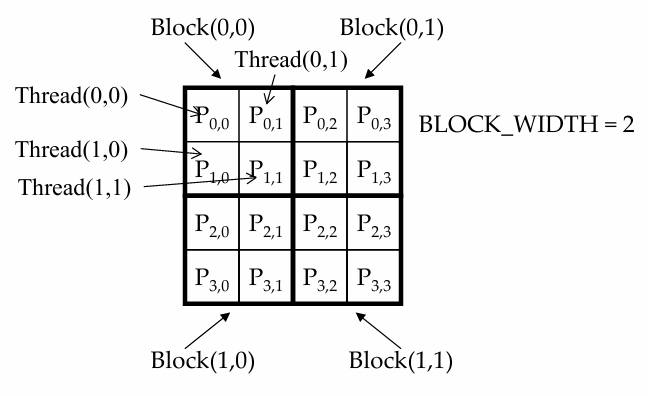
\includegraphics[width=0.6\textwidth]{figuresP/lesson_parallel_4_pag_36.png}
\end{center}
The code in App. \ref{app:matrix_example_cuda} is fairly complicated and using some time to read it and understand how it works can be a useful exercise. However our main point of interest is as follows.

Using the GeForce MX330, I executed the multiplication of 2 1024x1024 matrices with a grid of 16x16 blocks and got the following output. 
\begin{Verbatim}
[Output of > MatrixMultiplication_global 1024 1024 1024]
CUDA malloc A: no error
Copy A to device: no error
CUDA malloc B: no error
Copy B to device: no error
CUDA malloc C: no error
Run kernel: no error
Time: 36.52512 ms
Copy C off of device: no error
\end{Verbatim}
The execution lasted about 36 ms. You can try to write (or find online) a serial version of the same operation and you will find that it might take 30 s to 1 min to run with a normal CPU \footnote{The serial version of this code was run in class but I couldn't find it on the E-Learning platform of the course. However there are thousands of C programs for matrix multiplication published online that you can use as proof.}. Here the speed up is massive, about $10^4$. This is the most classic example of a \textbf{computation bound problem}: the latency of the CPU execution is due to the enormous amount of operations needed to complete the task, so using the GPU has given us an enormous boost.

We might already be happy with that, but it is possible to do better. For the multiplication of 2 NxN matrices we need N multiplications and N sums for each of the N elements in the result, for a total of 2N$^2$ FLOPs. However, once our matrices have been copied on the global memory of the device, it is necessary to access such memory 2N times for each element in order to retrieve the row and the column and compute the dot product. In other words, we also need 2N$^2$ memory accesses and our ratio "computation-to-memory access" is exactly 1. Let's consider this numerical example:
\begin{itemize}
    \item[-] Assume 100x100 matrices with single precision floating point elements (4 bytes).
    \item[-] In the GeForce MX330 the memory bandwidth (the amount of data that can be transferred from the global memory to the processor) is 56 GB/s.
    \item[-] How many operands (numbers to sum) per second can we load? \\ $56 \ \text{GB} / (2\text{N} \ \cdot \ 4 \ \text{bytes})=7\cdot10^9 \quad \Rightarrow$ \\
    We can load 7 billion operands per second.
    \item[-] Having a ratio "computation-to-memory access" of 1, that means that we can only execute 7 GFLOPS, which is very far from the 1.22 TFLOPS potential of the device!
\end{itemize}
In other words, our GPU could execute much more operations per second but it is constrained by the small memory bandwidth which slows everything down. The next step will be to escape (or at least limit) this memory access bottleneck.

That is exactly what the code \underline{MatrixMultiplication\_local.cu} in App. \ref{app:matrix_example_cuda} does. This is a very complicated example and we won't analyse it line by line, we will just explain the general principle behind it. 

As said, the global memory is a piece of hardware that is separated from the actual processor, but every multiprocessor also has an on-chip memory: the shared memory. Every thread run on the multiprocessor can write on and read the shared memory, and accessing it is orders of magnitude faster than the global one due to its physical vicinity to the cores. On the counter, it can contain only kilobytes or a few megabytes (for more modern devices) of information. That means that if we wanted to exploit the shared memory for our computations, there would not be enough space to copy all the matrices inside it. The trick is then to copy only a part of the data in the shared memory and then keep it there until all the operations that include it are completed. How do we apply that to matrices?

Take a look at the following figure that shows the multiplication $N \times M=P$. It becomes clear that once the line $M_{0,i}$ is copied in the shared memory, it can be rapidly used by all the threads that compute the elements in the line $P_{0,i}$, limiting the accessing to the global one.

\begin{center}
    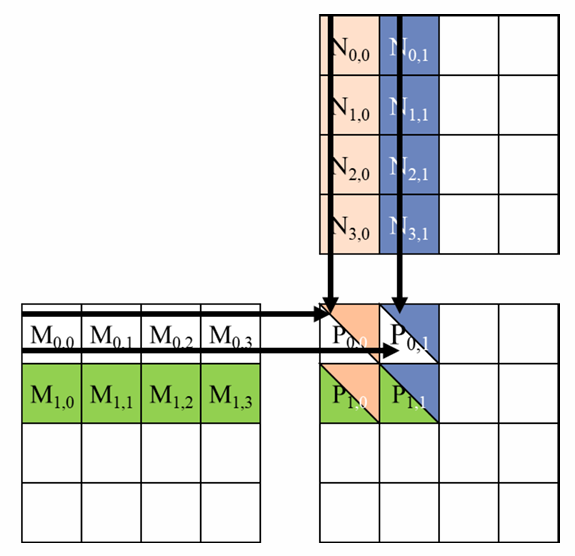
\includegraphics[width=0.35\textwidth]{figuresP/lesson_parallel_4_pag_37.png}
\end{center}

\begin{figure}[htbp]
    \begin{minipage}[c]{0.55\textwidth}
    Here is is the workflow applied in the complete code in App. \ref{app:matrix_example_cuda}:
    \begin{enumerate}
        \item Identify a “tile” of global memory contents that are accessed by multiple threads (e.g. a line of the M matrix);
        \item Load the tile from global memory into on-chip memory;
        \item Use barrier synchronization to make sure that all threads are ready to start the current execution phase (\texttt{\_\_syncthreads()});
        \item Have multiple threads access their data from the on-chip memory (and copy what's needed from the global one);
        \item Use barrier synchronization to make sure that all threads have completed the current phase;
        \item Move on to the next tile.
    \end{enumerate}
    \end{minipage}\hfill 
    \begin{minipage}[c]{0.4\textwidth}
        \centering
        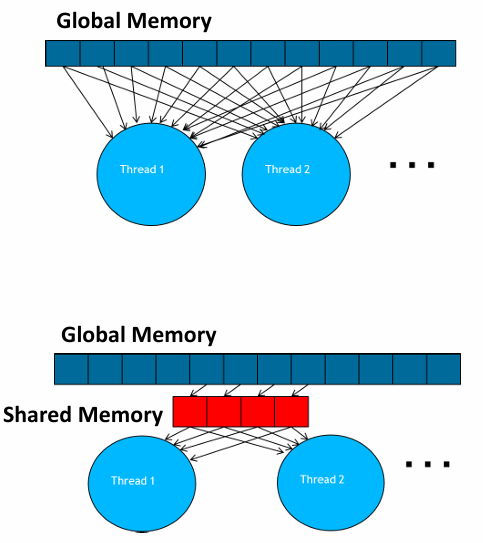
\includegraphics[width=\textwidth]{figuresP/lesson_parallel_4_pag_39.png}
    \end{minipage}
\end{figure} 
With this kind of implementation, the execution time was reduced to about 16 ms (more complex problems can experience much higher speed ups).

\hrulefill

\subsection{Note: Memory coalescing}

Another important concept that can be used for parallel programming is \textbf{memory coalescing}. We will not be implementing in with a practical example, but it is useful to know what it is.

In reality, both the global and shared memory (and even the RAM) are organized in groups called \textbf{bursts}: each address space is partitioned into burst sections and whenever a location is accessed, all other locations in the same section are also delivered to the processor, whether you like it or not. In practice, we have at least a 4GB address space, with burst section sizes of 128-bytes or more. If all accessed locations fall into the same burst section, only one RAM request will be made, and the access is said to be fully coalesced. When the accessed locations spread across burst section boundaries, coalescing fails. This means that in GPU computing it is useful (if possible) to organize our data in such a way that threads inside the same block will act on the same burst, in order to limit the number of memory accesses using coalescence. Otherwise some of the bytes transferred will not be used during the execution. The following figure shows a simple situation of a memory space organized in 4 burst of 4 bites and an example of coalesced memory load and un-coalesced memory load. 

\begin{center}
    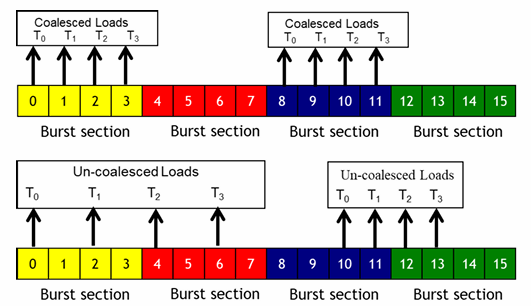
\includegraphics[width=0.5\textwidth]{figuresP/lesson_parallel_4_pag_46.png}
\end{center}

As a practical example, consider a standard matrix multiplication $A \times B = C$. As shown in the following figure, memory accesses to matrix B can easily be mapped sequentially along the rows ($B_{0,0}, B_{0,1}, \dots$), perfectly aligning with the contiguous burst sections and resulting in coalesced loads (top). Conversely, threads accessing matrix A must read down the columns ($A_{0,0}, A_{1,0}, \dots$). Because these values are scattered across different rows, each thread is forced to fetch data from an entirely different burst section, leading to un-coalesced access (bottom). A standard solution to speed up execution is to transpose the un-coalesced matrix (in this case, matrix A) prior to the operation. By reorganizing the data in memory, we allow the GPU to fetch the data in single and fully coalesced bursts.

\begin{center}
    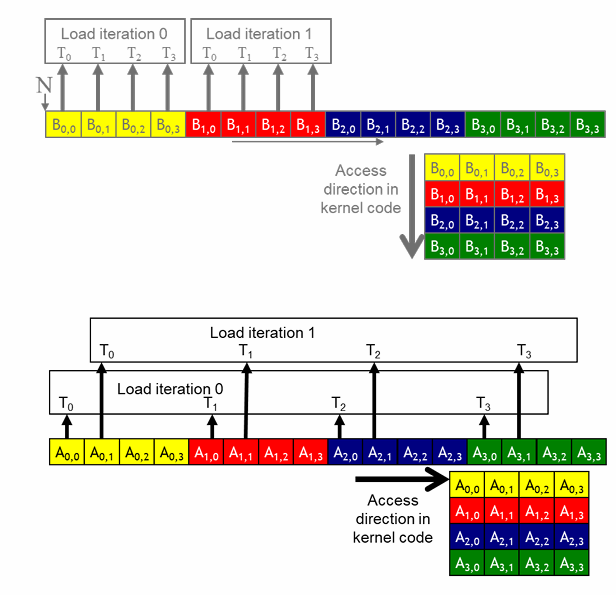
\includegraphics[width=0.5\textwidth]{figuresP/lesson_parallel_4_pag_47.png}
\end{center}

\begin{comment}
\subsection{HelloWorld}
HelloWorld example. Try to change the kernel launch parameters. Compile with \texttt{nvcc HelloWorld.cu -o HelloWorld -arch=compute\_35}.

\input{pygments/figuresP/lesson_parallel_4_pag_31.png}

\subsection{Vector Sum (Serial)}
We want to sum two vectors of 1048576 elements each. First we will try to write a "serial" version of the code. Due to the presence of cuda functions to measure the time, this code must be compiled with \texttt{nvcc}. Time: 4.4 ms (on GTX 650).

\input{pygments/figuresP/lesson_parallel_4_pag_32.png}

\subsection{Vector Sum (parallel)}
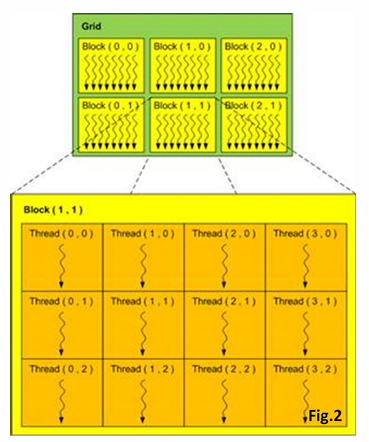
\includegraphics[width=0.6\textwidth]{figuresP/lesson_parallel_4_pag_33.png}

Let's try to parallelize, by using several blocks. Remember to copy data from host to device and results back. The results is not what we expect. Why? Time: 17.3 ms !!!

\input{pygments/figuresP/lesson_parallel_4_pag_33.png}

\subsection{Vector Sum (parallel): $2^\circ$ attempt}
Then let's try to use one single block and N Threads. Time = 0.01 ms, SpeedUp = 370. Uhmmmmmmmmmmmm. A reasonable speedup is around 100 or less. Try to print something: the results, the error code. Try to have a look to the maximum size of threads per block.

\input{pygments/figuresP/lesson_parallel_4_pag_34.png}

\subsection{Vector Sum (parallel): final attempt}
\includegraphics[width=0.6\textwidth]{figuresP/lesson_parallel_4_pag_35.png}

Use both threads and blocks. The total number of threads must be equal to the number of elements in the vectors. Define an "index" by using the block/thread identifier. The kernel must be adapted to this structure. Time = 0.48 ms (without errors).

\input{pygments/figuresP/lesson_parallel_4_pag_35.png}

\subsection{Matrix Multiplication}
Assume you want to multiply two large matrices. Use a 2D structure of threads and blocks. Each thread computes one element of the matrix. Use the blocks to subdivide the matrix in sub-blocks.

\input{pygments/figuresP/lesson_parallel_4_pag_36.png}

\subsection{Limitations to computing power}
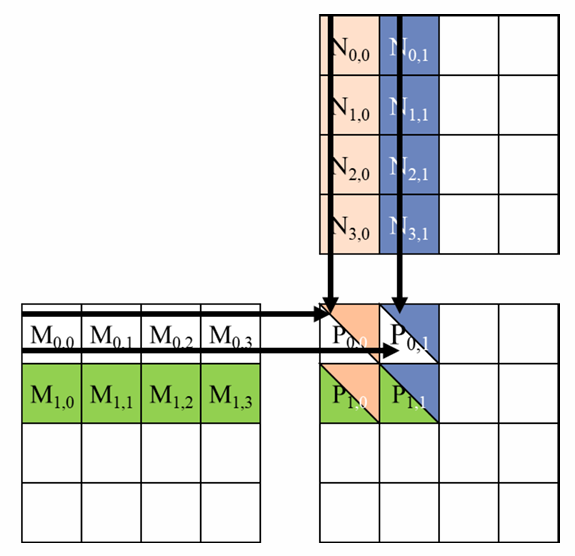
\includegraphics[width=0.6\textwidth]{figuresP/lesson_parallel_4_pag_37.png}

A lot of accesses to memory are required: for each element computed we need 2N global memory accesses, and 2N operations (N multiplications and N sums). The compute-to-global-memory-access ratio is 1:1.
In the K20 the memory bandwidth is 200 GB/s. Assuming $100\times100$ matrices, how many operands per second can we load? $200 \text{ GB} / (2N * 4\text{ bytes}) = 25 \text{ Goperands/s}$. Since the ratio is limited to 1, this means that the computing throughput is 25 GFlops, which is very far from the 3.5 TFlops capability of the board!

\subsection{Shared Memory}
\includegraphics[width=0.6\textwidth]{figuresP/lesson_parallel_4_pag_38.png}

Shared memory is a special type of memory whose contents are explicitly defined and used in the kernel source code. There is one in each SM, and it is accessed at much higher speed (in both latency and throughput) than global memory. The scope of access and sharing is restricted to thread blocks. Its lifetime corresponds to the thread block: contents will disappear after the corresponding thread block finishes execution. It is accessed by memory load/store instructions and acts as a form of scratchpad memory in computer architecture.

\begin{table}[H]
\centering
\begin{tabular}{|l|l|l|l|}
\hline
\textbf{Variable declaration} & \textbf{Memory} & \textbf{Scope} & \textbf{Lifetime} \\ \hline
\texttt{int LocalVar;} & register & thread & thread \\ \hline
\texttt{\_\_device\_\_ \_\_shared\_\_ int SharedVar;} & shared & block & block \\ \hline
\texttt{\_\_device\_\_ int GlobalVar;} & global & grid & application \\ \hline
\texttt{\_\_device\_\_ \_\_constant\_\_ int ConstantVar;} & constant & grid & application \\ \hline
\end{tabular}
\end{table}

\subsection{Shared memory for Matrix Multiplication}
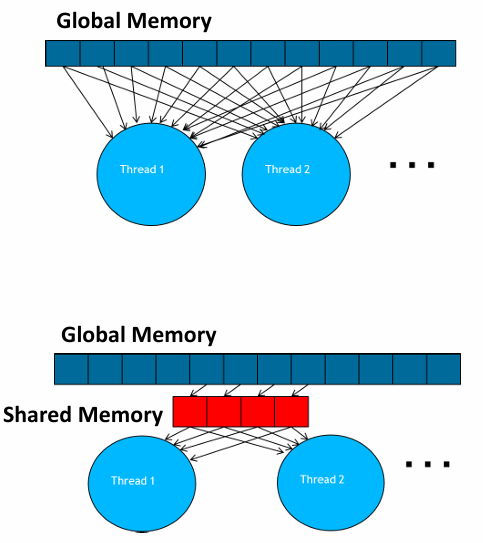
\includegraphics[width=0.6\textwidth]{figuresP/lesson_parallel_4_pag_39.png}

Identify a "tile" of global memory contents that are accessed by multiple threads. Load the tile from global memory into on-chip shared memory. Use barrier synchronization to make sure that all threads are ready to start the phase. Have the multiple threads access their data from the on-chip memory. Use barrier synchronization again to ensure that all threads have completed the current phase before moving on to the next tile.

\subsection{Shared memory: phase 0 load for block (0,0)}
During Phase 0 load, threads load tiles from matrices M and N into shared memory. For example, $thread_{0,0}$ loads $M_{0,0}$ and $N_{0,0}$.

\subsection{Shared memory: phase 0 use block (0,0)}
During Phase 0 use, threads compute partial products using the shared memory tiles. For example, $PValue_{0,0}$ accumulates $Mds_{0,0} * Nds_{0,0} + Mds_{0,1} * Nds_{1,0}$.

\subsection{Execution phases}
Threads execute loads and mathematical operations simultaneously in phases.
\textbf{Phase 0}:
$thread_{0,0}$ loads $M_{0,0}$ into $Mds_{0,0}$ and $N_{0,0}$ into $Nds_{0,0}$. It then computes $PValue_{0,0} += Mds_{0,0} * Nds_{0,0} + Mds_{0,1} * Nds_{1,0}$.
\textbf{Phase 1}:
$thread_{0,0}$ loads $M_{0,2}$ and $N_{2,0}$. It computes the next partial sum for $PValue_{0,0}$. This continues across all threads ($thread_{0,1}$, $thread_{1,0}$, $thread_{1,1}$) through time.

\subsection{Synchronization}
Synchronize all threads in a block using \texttt{\_\_syncthreads()}. All threads in the same block must reach the \texttt{\_\_syncthreads()} before any of them can move on. This is best used to coordinate phased execution in tiled algorithms, ensuring that all elements of a tile are loaded at the beginning of a phase, and that all elements of a tile are consumed at the end of a phase.

\subsection{MatrixMultiplication code}
HOST and GPU implementation for matrix multiplication utilizing shared memory.

\input{pygments/figuresP/lesson_parallel_4_pag_44.png}
\input{pygments/figuresP/lesson_parallel_4_pag_45.png}

\subsection{Memory coalescing}
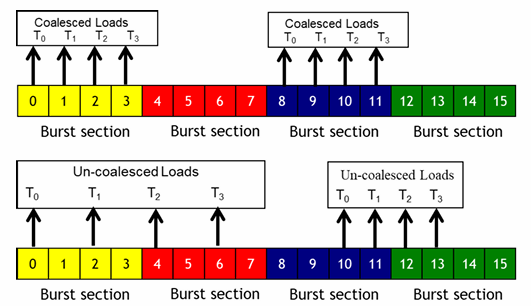
\includegraphics[width=0.6\textwidth]{figuresP/lesson_parallel_4_pag_46.png}

Each address space is partitioned into burst sections. Whenever a location is accessed, all other locations in the same section are also delivered to the processor. In practice, we have at least a 4GB address space, with burst section sizes of 128-bytes or more.
If all accessed locations fall into the same burst section, only one DRAM request will be made and the access is fully coalesced. When the accessed locations spread across burst section boundaries, coalescing fails. Multiple DRAM requests are made, and some of the bytes transferred are not used by the threads.

\subsection{Memory access in Matrix Multiplication}
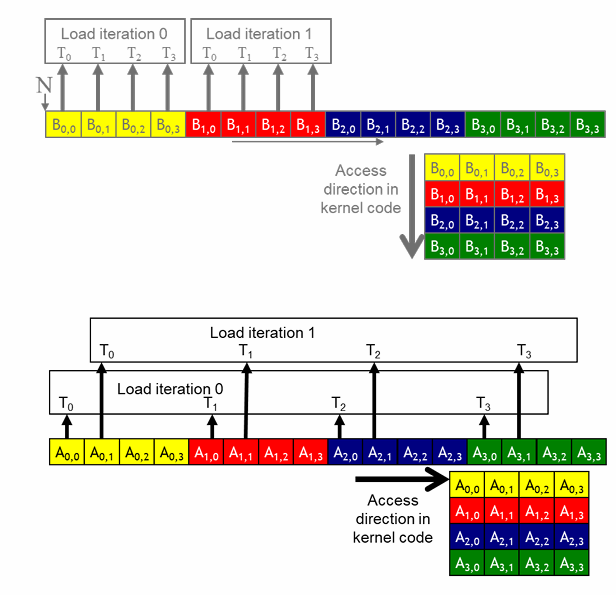
\includegraphics[width=0.6\textwidth]{figuresP/lesson_parallel_4_pag_47.png}

When loading rows/columns from matrices A and B: access to matrix B is coalesced because threads access contiguous memory locations. Access to matrix A is not coalesced because threads access data column-wise, spanning across different burst sections.

\subsection{For Hands-on next lecture}
We will use Colab (\url{https://colab.research.google.com}), requiring a Google account. It is based on Jupyter Notebook. Read the introduction on the first page. Colab allows you to use machines with GPU (and also TPU).

\subsection{Bibliography}
\textbf{Parallel programming:}
\begin{itemize}
    \item "The source book of parallel computing" (Dongarra et al.) - Morgan Kaufmann ed. (2003)
    \item "Introduction to parallel programming" (Grama-Gupta-Karypis-Kumar)
\end{itemize}
\textbf{Parallel processing in python:}
\begin{itemize}
    \item \url{https://docs.python.org/2/library/multiprocessing.html}
    \item \url{https://docs.python.org/3/library/threading.html}
\end{itemize}
\textbf{GPU online resources:}
\begin{itemize}
    \item \url{https://docs.nvidia.com/cuda/index.html}
    \item \url{https://docs.nvidia.com/pdf/CUDA_C_Programming_Guide.pdf}
    \item \url{https://docs.nvidia.com/pdf/CUDA_C_Best_Practices_Guide.pdf}
    \item \url{https://hgpu.org/} (collection of tutorials and articles)
\end{itemize}
\textbf{GPU books:}
\begin{itemize}
    \item "GPU Computing and Applications" (Yiju Cai) - Springer
    \item "Multicore and gpu programming: an integrated approach" (Barlas) - Morgan Kaufmann
    \item "Cuda by Example" (Sanders) - Addison-Wesley
    \item "Professional Cuda C programming" (Cheng et al.) - Wrox
\end{itemize}
\textbf{GPU in Python:}
\begin{itemize}
    \item \url{https://wish4book.com/education/5410-hands-on-gpu-computing-with-python.html}
    \item \url{https://documen.tician.de/pycuda/}
\end{itemize}

\subsection{Appendix: Purpose of this addendum}
The purpose of this addendum is to present some classic problems that can be addressed with GPU. The kernels proposed are deliberately incomplete (and sometimes also wrong). As an assignment, try to complete one or more of the proposed solutions to have a working kernel. Then try to include this kernel in a python code by using pyCUDA. Try to measure the timing of your implementation with respect to a simpler implementation or with respect to the serial version to show the speedup introduced by your work.

\subsection{Histograms}
\includegraphics[width=0.6\textwidth]{figuresP/lesson_parallel_4_pag_52.png}

Building histograms is a method for extracting features and patterns from large data sets. Typical applications include standard decryption methods, feature extraction for object recognition in images, search for decays in High Energy Physics, and correlating heavenly object movements in astrophysics. For each element in the data set, use the value to identify a "bin counter" to increment.

\subsection{Simple Histograms algorithm}
\includegraphics[width=0.6\textwidth]{figuresP/lesson_parallel_4_pag_53.png}

Partition the input into sections. Have each thread take a section of the input. Each thread iterates through its section. For each letter, increment the appropriate bin counter.

\subsection{Limits to "partitioning"}
\includegraphics[width=0.6\textwidth]{figuresP/lesson_parallel_4_pag_54.png}

Sectioned partitioning results in poor memory access efficiency. Adjacent threads do not access adjacent memory locations, therefore accesses are not coalesced and DRAM bandwidth is poorly utilized.

\subsection{Interleaved input access}
\includegraphics[width=0.6\textwidth]{figuresP/lesson_parallel_4_pag_55.png}

Change to interleaved partitioning. All threads process a contiguous section of elements. They all move to the next section and repeat. This way, memory accesses are coalesced. In this case, the logic partitioning is a little bit more complicated but the access to the memory is very efficient.

\subsection{Data races}
\includegraphics[width=0.6\textwidth]{figuresP/lesson_parallel_4_pag_56.png}

Interleaving solves the problem of access to the memory in input, but writing the histogram is still problematic. Different threads write at the same time in the same location in the output memory space. We have already seen the problem of data races in python multiprocessing. In GPU programming, it is not "natural" to use semaphores because the code is essentially SIMD.

\subsection{Atomic Operations}
A read-modify-write operation performed by a single hardware instruction on a memory location address. It reads the old value, calculates a new value, and writes the new value to the location. The hardware ensures that no other threads can perform another read-modify-write operation on the same location until the current atomic operation is complete. Any other threads attempting to access the same location will be held in a queue, forcing serial operations on that specific memory cell. Performed by calling intrinsic functions (e.g., atomic add, sub, inc, dec, min, max, exch, CAS).
For example, \texttt{atomicAdd(int* address, int val)} reads the 32-bit word \texttt{old} from the location pointed to by \texttt{address}, computes \texttt{old + val}, stores the result back, and returns \texttt{old+val}.

\subsection{Histograms kernel}
Assignment: Follow the example. Notice the stride and the use of \texttt{atomicAdd()}. Write the host code in Python and include the kernel by using \texttt{SourceModule} of pyCUDA. Define the "histogram" with the correct dimensions and plot it with matplotlib.

\input{pygments/figuresP/lesson_parallel_4_pag_58.png}

\subsection{Convolution}
The convolution is widely used in several fields (audio, image processing). It is the base of "stencil computing". A convolution is a filter that transforms signal or pixel values into more desirable values. Gaussian filters can be used to sharpen boundaries and edges of objects in images. Some filters smooth out the signal values so that one can see the big-picture trend.

\subsection{Computational definition of Convolution}
\includegraphics[width=0.6\textwidth]{figuresP/lesson_parallel_4_pag_60.png}

An array operation where each output data element is a weighted sum of a collection of neighboring input elements. The weights used are defined by an input mask array (convolution mask). The value pattern of the mask array elements defines the type of filtering done (e.g., Image blurring).

\subsection{1D Convolution example}
Example of calculating element $P[2]$ using inputs from $N$ and mask $M$: $P[2] = N[0]*M[0] + N[1]*M[1] + N[2]*M[2] + N[3]*M[3] + N[4]*M[4]$.

\subsection{1D convolution: boundaries}
\includegraphics[width=0.6\textwidth]{figuresP/lesson_parallel_4_pag_62.png}

Calculation of output elements near the boundaries (beginning and end) of the array need to deal with "ghost" elements. Different policies exist for this (e.g., using 0, replicates of boundary values, etc.).

\subsection{A simple stencil kernel}
\input{pygments/figuresP/lesson_parallel_4_pag_63.png}

\subsection{Calculation of adjacent output elements}
Calculation of adjacent output elements involves shared input elements. For example, $N[2]$ is used in the calculation of $P[0]$, $P[1]$, $P[2]$, $P[3]$, and $P[4]$ (assuming a 1D convolution mask of width 5). We can load all the input elements required by all threads in a block into the shared memory to reduce global memory accesses.

\subsection{Subdivide the input array in tiles}
Subdivide the input array in tiles. Each tile is $nP$ elements large, where $nP$ is the number of threads in a block. Cache data in shared memory. All the threads in a block will copy one element into the shared memory from the global memory. $2 * \text{radius}$ extra elements (where radius is the width of the halo around the $nP$ elements) are also included to handle boundaries.

\subsection{Shared memory stencil 1D}
\input{pygments/figuresP/lesson_parallel_4_pag_66.png}

\subsection{Parallel reduction}
\includegraphics[width=0.6\textwidth]{figuresP/lesson_parallel_4_pag_67.png}

A large class of algorithms on large data sets are based on the idea to reduce the amount of interesting information. Google and Hadoop MapReduce frameworks support this strategy. There is no required order for processing elements in a data set (associative and commutative operations like Max, Min, Sum, Product). You partition the data set into smaller chunks, have each thread process a chunk, and then use a reduction tree to summarize the results from each chunk into the final answer.

\subsection{Simple Parallel reduction tree}
In a simple parallelization, each operation is performed by a different task. For $N$ initial values, the tree performs $(N-1)$ operations in $\log(N)$ parallel steps. The average parallelization per step is $(N-1)/\log(N)$. For example, if $N=1000000$, we have on average 50000 parallel workers, but the peak requires 500000 parallel workers (in step 1), while the last step needs only one worker. This represents a very inefficient use of parallel resources, particularly for SIMD. It's a good idea to rethink the parallel structure to efficiently reuse the computing units.

\subsection{Parallel sum with shared memory}
\includegraphics[width=0.6\textwidth]{figuresP/lesson_parallel_4_pag_69.png}

Recursively halve the number of threads, adding two values per thread in each step. This takes $\log(n)$ steps for $n$ elements and requires $n/2$ threads. This assumes an in-place reduction using shared memory. The original vector is in device global memory; shared memory is used to hold a partial sum vector. Each step brings the partial sum closer to the total sum, which will ultimately be in element 0. Thread block size limits $n$ to be $\le 2048$. This greatly reduces global memory traffic.

\subsection{Additional assignment}
Try to write the GPU version of the assignment proposed in the processing in Python lecture. Measure the speedup with respect to multithreading and multiprocessing and produce a plot to compare the results.

\subsection{License}
\includegraphics[width=0.6\textwidth]{figuresP/lesson_parallel_4_pag_71.png}

Part of the material used for this presentation comes from the "GPU Teaching KIT" licensed by NVIDIA and University of Illinois, and has been used and modified according to Creative Commons attribution non-commercial 4.0.

\end{comment}